\def\year{2020}\relax
%File: formatting-instruction.tex
\documentclass[letterpaper]{article} % DO NOT CHANGE THIS
\usepackage{aaai20}  % DO NOT CHANGE THIS
\usepackage{times}  % DO NOT CHANGE THIS
\usepackage{helvet} % DO NOT CHANGE THIS
\usepackage{courier}  % DO NOT CHANGE THIS
\usepackage[hyphens]{url}  % DO NOT CHANGE THIS
\usepackage{graphicx} % DO NOT CHANGE THIS
\urlstyle{rm} % DO NOT CHANGE THIS
\def\UrlFont{\rm}  % DO NOT CHANGE THIS
\usepackage{graphicx}  % DO NOT CHANGE THIS
\frenchspacing  % DO NOT CHANGE THIS
\setlength{\pdfpagewidth}{8.5in}  % DO NOT CHANGE THIS
\setlength{\pdfpageheight}{11in}  % DO NOT CHANGE THIS

%====================================================================================
%%%%% NEW MATH DEFINITIONS %%%%%

\usepackage{amsmath,amsfonts,bm}

% Mark sections of captions for referring to divisions of figures
\newcommand{\figleft}{{\em (Left)}}
\newcommand{\figcenter}{{\em (Center)}}
\newcommand{\figright}{{\em (Right)}}
\newcommand{\figtop}{{\em (Top)}}
\newcommand{\figbottom}{{\em (Bottom)}}
\newcommand{\captiona}{{\em (a)}}
\newcommand{\captionb}{{\em (b)}}
\newcommand{\captionc}{{\em (c)}}
\newcommand{\captiond}{{\em (d)}}

% Highlight a newly defined term
\newcommand{\newterm}[1]{{\bf #1}}


% Figure reference, lower-case.
\def\figref#1{figure~\ref{#1}}
% Figure reference, capital. For start of sentence
\def\Figref#1{Figure~\ref{#1}}
\def\twofigref#1#2{figures \ref{#1} and \ref{#2}}
\def\quadfigref#1#2#3#4{figures \ref{#1}, \ref{#2}, \ref{#3} and \ref{#4}}
% Section reference, lower-case.
\def\secref#1{section~\ref{#1}}
% Section reference, capital.
\def\Secref#1{Section~\ref{#1}}
% Reference to two sections.
\def\twosecrefs#1#2{sections \ref{#1} and \ref{#2}}
% Reference to three sections.
\def\secrefs#1#2#3{sections \ref{#1}, \ref{#2} and \ref{#3}}
% Reference to an equation, lower-case.
\def\eqref#1{equation~\ref{#1}}
% Reference to an equation, upper case
\def\Eqref#1{Equation~\ref{#1}}
% A raw reference to an equation---avoid using if possible
\def\plaineqref#1{\ref{#1}}
% Reference to a chapter, lower-case.
\def\chapref#1{chapter~\ref{#1}}
% Reference to an equation, upper case.
\def\Chapref#1{Chapter~\ref{#1}}
% Reference to a range of chapters
\def\rangechapref#1#2{chapters\ref{#1}--\ref{#2}}
% Reference to an algorithm, lower-case.
\def\algref#1{algorithm~\ref{#1}}
% Reference to an algorithm, upper case.
\def\Algref#1{Algorithm~\ref{#1}}
\def\twoalgref#1#2{algorithms \ref{#1} and \ref{#2}}
\def\Twoalgref#1#2{Algorithms \ref{#1} and \ref{#2}}
% Reference to a part, lower case
\def\partref#1{part~\ref{#1}}
% Reference to a part, upper case
\def\Partref#1{Part~\ref{#1}}
\def\twopartref#1#2{parts \ref{#1} and \ref{#2}}

\def\ceil#1{\lceil #1 \rceil}
\def\floor#1{\lfloor #1 \rfloor}
\def\1{\bm{1}}
\newcommand{\train}{\mathcal{D}}
\newcommand{\valid}{\mathcal{D_{\mathrm{valid}}}}
\newcommand{\test}{\mathcal{D_{\mathrm{test}}}}

\def\eps{{\epsilon}}


% Random variables
\def\reta{{\textnormal{$\eta$}}}
\def\ra{{\textnormal{a}}}
\def\rb{{\textnormal{b}}}
\def\rc{{\textnormal{c}}}
\def\rd{{\textnormal{d}}}
\def\re{{\textnormal{e}}}
\def\rf{{\textnormal{f}}}
\def\rg{{\textnormal{g}}}
\def\rh{{\textnormal{h}}}
\def\ri{{\textnormal{i}}}
\def\rj{{\textnormal{j}}}
\def\rk{{\textnormal{k}}}
\def\rl{{\textnormal{l}}}
% rm is already a command, just don't name any random variables m
\def\rn{{\textnormal{n}}}
\def\ro{{\textnormal{o}}}
\def\rp{{\textnormal{p}}}
\def\rq{{\textnormal{q}}}
\def\rr{{\textnormal{r}}}
\def\rs{{\textnormal{s}}}
\def\rt{{\textnormal{t}}}
\def\ru{{\textnormal{u}}}
\def\rv{{\textnormal{v}}}
\def\rw{{\textnormal{w}}}
\def\rx{{\textnormal{x}}}
\def\ry{{\textnormal{y}}}
\def\rz{{\textnormal{z}}}

% Random vectors
\def\rvepsilon{{\mathbf{\epsilon}}}
\def\rvtheta{{\mathbf{\theta}}}
\def\rva{{\mathbf{a}}}
\def\rvb{{\mathbf{b}}}
\def\rvc{{\mathbf{c}}}
\def\rvd{{\mathbf{d}}}
\def\rve{{\mathbf{e}}}
\def\rvf{{\mathbf{f}}}
\def\rvg{{\mathbf{g}}}
\def\rvh{{\mathbf{h}}}
\def\rvu{{\mathbf{i}}}
\def\rvj{{\mathbf{j}}}
\def\rvk{{\mathbf{k}}}
\def\rvl{{\mathbf{l}}}
\def\rvm{{\mathbf{m}}}
\def\rvn{{\mathbf{n}}}
\def\rvo{{\mathbf{o}}}
\def\rvp{{\mathbf{p}}}
\def\rvq{{\mathbf{q}}}
\def\rvr{{\mathbf{r}}}
\def\rvs{{\mathbf{s}}}
\def\rvt{{\mathbf{t}}}
\def\rvu{{\mathbf{u}}}
\def\rvv{{\mathbf{v}}}
\def\rvw{{\mathbf{w}}}
\def\rvx{{\mathbf{x}}}
\def\rvy{{\mathbf{y}}}
\def\rvz{{\mathbf{z}}}

% Elements of random vectors
\def\erva{{\textnormal{a}}}
\def\ervb{{\textnormal{b}}}
\def\ervc{{\textnormal{c}}}
\def\ervd{{\textnormal{d}}}
\def\erve{{\textnormal{e}}}
\def\ervf{{\textnormal{f}}}
\def\ervg{{\textnormal{g}}}
\def\ervh{{\textnormal{h}}}
\def\ervi{{\textnormal{i}}}
\def\ervj{{\textnormal{j}}}
\def\ervk{{\textnormal{k}}}
\def\ervl{{\textnormal{l}}}
\def\ervm{{\textnormal{m}}}
\def\ervn{{\textnormal{n}}}
\def\ervo{{\textnormal{o}}}
\def\ervp{{\textnormal{p}}}
\def\ervq{{\textnormal{q}}}
\def\ervr{{\textnormal{r}}}
\def\ervs{{\textnormal{s}}}
\def\ervt{{\textnormal{t}}}
\def\ervu{{\textnormal{u}}}
\def\ervv{{\textnormal{v}}}
\def\ervw{{\textnormal{w}}}
\def\ervx{{\textnormal{x}}}
\def\ervy{{\textnormal{y}}}
\def\ervz{{\textnormal{z}}}

% Random matrices
\def\rmA{{\mathbf{A}}}
\def\rmB{{\mathbf{B}}}
\def\rmC{{\mathbf{C}}}
\def\rmD{{\mathbf{D}}}
\def\rmE{{\mathbf{E}}}
\def\rmF{{\mathbf{F}}}
\def\rmG{{\mathbf{G}}}
\def\rmH{{\mathbf{H}}}
\def\rmI{{\mathbf{I}}}
\def\rmJ{{\mathbf{J}}}
\def\rmK{{\mathbf{K}}}
\def\rmL{{\mathbf{L}}}
\def\rmM{{\mathbf{M}}}
\def\rmN{{\mathbf{N}}}
\def\rmO{{\mathbf{O}}}
\def\rmP{{\mathbf{P}}}
\def\rmQ{{\mathbf{Q}}}
\def\rmR{{\mathbf{R}}}
\def\rmS{{\mathbf{S}}}
\def\rmT{{\mathbf{T}}}
\def\rmU{{\mathbf{U}}}
\def\rmV{{\mathbf{V}}}
\def\rmW{{\mathbf{W}}}
\def\rmX{{\mathbf{X}}}
\def\rmY{{\mathbf{Y}}}
\def\rmZ{{\mathbf{Z}}}

% Elements of random matrices
\def\ermA{{\textnormal{A}}}
\def\ermB{{\textnormal{B}}}
\def\ermC{{\textnormal{C}}}
\def\ermD{{\textnormal{D}}}
\def\ermE{{\textnormal{E}}}
\def\ermF{{\textnormal{F}}}
\def\ermG{{\textnormal{G}}}
\def\ermH{{\textnormal{H}}}
\def\ermI{{\textnormal{I}}}
\def\ermJ{{\textnormal{J}}}
\def\ermK{{\textnormal{K}}}
\def\ermL{{\textnormal{L}}}
\def\ermM{{\textnormal{M}}}
\def\ermN{{\textnormal{N}}}
\def\ermO{{\textnormal{O}}}
\def\ermP{{\textnormal{P}}}
\def\ermQ{{\textnormal{Q}}}
\def\ermR{{\textnormal{R}}}
\def\ermS{{\textnormal{S}}}
\def\ermT{{\textnormal{T}}}
\def\ermU{{\textnormal{U}}}
\def\ermV{{\textnormal{V}}}
\def\ermW{{\textnormal{W}}}
\def\ermX{{\textnormal{X}}}
\def\ermY{{\textnormal{Y}}}
\def\ermZ{{\textnormal{Z}}}

% Vectors
\def\vzero{{\bm{0}}}
\def\vone{{\bm{1}}}
\def\vmu{{\bm{\mu}}}
\def\vtheta{{\bm{\theta}}}
\def\va{{\bm{a}}}
\def\vb{{\bm{b}}}
\def\vc{{\bm{c}}}
\def\vd{{\bm{d}}}
\def\ve{{\bm{e}}}
\def\vf{{\bm{f}}}
\def\vg{{\bm{g}}}
\def\vh{{\bm{h}}}
\def\vi{{\bm{i}}}
\def\vj{{\bm{j}}}
\def\vk{{\bm{k}}}
\def\vl{{\bm{l}}}
\def\vm{{\bm{m}}}
\def\vn{{\bm{n}}}
\def\vo{{\bm{o}}}
\def\vp{{\bm{p}}}
\def\vq{{\bm{q}}}
\def\vr{{\bm{r}}}
\def\vs{{\bm{s}}}
\def\vt{{\bm{t}}}
\def\vu{{\bm{u}}}
\def\vv{{\bm{v}}}
\def\vw{{\bm{w}}}
\def\vx{{\bm{x}}}
\def\vy{{\bm{y}}}
\def\vz{{\bm{z}}}

% Elements of vectors
\def\evalpha{{\alpha}}
\def\evbeta{{\beta}}
\def\evepsilon{{\epsilon}}
\def\evlambda{{\lambda}}
\def\evomega{{\omega}}
\def\evmu{{\mu}}
\def\evpsi{{\psi}}
\def\evsigma{{\sigma}}
\def\evtheta{{\theta}}
\def\eva{{a}}
\def\evb{{b}}
\def\evc{{c}}
\def\evd{{d}}
\def\eve{{e}}
\def\evf{{f}}
\def\evg{{g}}
\def\evh{{h}}
\def\evi{{i}}
\def\evj{{j}}
\def\evk{{k}}
\def\evl{{l}}
\def\evm{{m}}
\def\evn{{n}}
\def\evo{{o}}
\def\evp{{p}}
\def\evq{{q}}
\def\evr{{r}}
\def\evs{{s}}
\def\evt{{t}}
\def\evu{{u}}
\def\evv{{v}}
\def\evw{{w}}
\def\evx{{x}}
\def\evy{{y}}
\def\evz{{z}}

% Matrix
\def\mA{{\bm{A}}}
\def\mB{{\bm{B}}}
\def\mC{{\bm{C}}}
\def\mD{{\bm{D}}}
\def\mE{{\bm{E}}}
\def\mF{{\bm{F}}}
\def\mG{{\bm{G}}}
\def\mH{{\bm{H}}}
\def\mI{{\bm{I}}}
\def\mJ{{\bm{J}}}
\def\mK{{\bm{K}}}
\def\mL{{\bm{L}}}
\def\mM{{\bm{M}}}
\def\mN{{\bm{N}}}
\def\mO{{\bm{O}}}
\def\mP{{\bm{P}}}
\def\mQ{{\bm{Q}}}
\def\mR{{\bm{R}}}
\def\mS{{\bm{S}}}
\def\mT{{\bm{T}}}
\def\mU{{\bm{U}}}
\def\mV{{\bm{V}}}
\def\mW{{\bm{W}}}
\def\mX{{\bm{X}}}
\def\mY{{\bm{Y}}}
\def\mZ{{\bm{Z}}}
\def\mBeta{{\bm{\beta}}}
\def\mPhi{{\bm{\Phi}}}
\def\mLambda{{\bm{\Lambda}}}
\def\mSigma{{\bm{\Sigma}}}

% Tensor
\DeclareMathAlphabet{\mathsfit}{\encodingdefault}{\sfdefault}{m}{sl}
\SetMathAlphabet{\mathsfit}{bold}{\encodingdefault}{\sfdefault}{bx}{n}
\newcommand{\tens}[1]{\bm{\mathsfit{#1}}}
\def\tA{{\tens{A}}}
\def\tB{{\tens{B}}}
\def\tC{{\tens{C}}}
\def\tD{{\tens{D}}}
\def\tE{{\tens{E}}}
\def\tF{{\tens{F}}}
\def\tG{{\tens{G}}}
\def\tH{{\tens{H}}}
\def\tI{{\tens{I}}}
\def\tJ{{\tens{J}}}
\def\tK{{\tens{K}}}
\def\tL{{\tens{L}}}
\def\tM{{\tens{M}}}
\def\tN{{\tens{N}}}
\def\tO{{\tens{O}}}
\def\tP{{\tens{P}}}
\def\tQ{{\tens{Q}}}
\def\tR{{\tens{R}}}
\def\tS{{\tens{S}}}
\def\tT{{\tens{T}}}
\def\tU{{\tens{U}}}
\def\tV{{\tens{V}}}
\def\tW{{\tens{W}}}
\def\tX{{\tens{X}}}
\def\tY{{\tens{Y}}}
\def\tZ{{\tens{Z}}}


% Graph
\def\gA{{\mathcal{A}}}
\def\gB{{\mathcal{B}}}
\def\gC{{\mathcal{C}}}
\def\gD{{\mathcal{D}}}
\def\gE{{\mathcal{E}}}
\def\gF{{\mathcal{F}}}
\def\gG{{\mathcal{G}}}
\def\gH{{\mathcal{H}}}
\def\gI{{\mathcal{I}}}
\def\gJ{{\mathcal{J}}}
\def\gK{{\mathcal{K}}}
\def\gL{{\mathcal{L}}}
\def\gM{{\mathcal{M}}}
\def\gN{{\mathcal{N}}}
\def\gO{{\mathcal{O}}}
\def\gP{{\mathcal{P}}}
\def\gQ{{\mathcal{Q}}}
\def\gR{{\mathcal{R}}}
\def\gS{{\mathcal{S}}}
\def\gT{{\mathcal{T}}}
\def\gU{{\mathcal{U}}}
\def\gV{{\mathcal{V}}}
\def\gW{{\mathcal{W}}}
\def\gX{{\mathcal{X}}}
\def\gY{{\mathcal{Y}}}
\def\gZ{{\mathcal{Z}}}

% Sets
\def\sA{{\mathbb{A}}}
\def\sB{{\mathbb{B}}}
\def\sC{{\mathbb{C}}}
\def\sD{{\mathbb{D}}}
% Don't use a set called E, because this would be the same as our symbol
% for expectation.
\def\sF{{\mathbb{F}}}
\def\sG{{\mathbb{G}}}
\def\sH{{\mathbb{H}}}
\def\sI{{\mathbb{I}}}
\def\sJ{{\mathbb{J}}}
\def\sK{{\mathbb{K}}}
\def\sL{{\mathbb{L}}}
\def\sM{{\mathbb{M}}}
\def\sN{{\mathbb{N}}}
\def\sO{{\mathbb{O}}}
\def\sP{{\mathbb{P}}}
\def\sQ{{\mathbb{Q}}}
\def\sR{{\mathbb{R}}}
\def\sS{{\mathbb{S}}}
\def\sT{{\mathbb{T}}}
\def\sU{{\mathbb{U}}}
\def\sV{{\mathbb{V}}}
\def\sW{{\mathbb{W}}}
\def\sX{{\mathbb{X}}}
\def\sY{{\mathbb{Y}}}
\def\sZ{{\mathbb{Z}}}

% Entries of a matrix
\def\emLambda{{\Lambda}}
\def\emA{{A}}
\def\emB{{B}}
\def\emC{{C}}
\def\emD{{D}}
\def\emE{{E}}
\def\emF{{F}}
\def\emG{{G}}
\def\emH{{H}}
\def\emI{{I}}
\def\emJ{{J}}
\def\emK{{K}}
\def\emL{{L}}
\def\emM{{M}}
\def\emN{{N}}
\def\emO{{O}}
\def\emP{{P}}
\def\emQ{{Q}}
\def\emR{{R}}
\def\emS{{S}}
\def\emT{{T}}
\def\emU{{U}}
\def\emV{{V}}
\def\emW{{W}}
\def\emX{{X}}
\def\emY{{Y}}
\def\emZ{{Z}}
\def\emSigma{{\Sigma}}

% entries of a tensor
% Same font as tensor, without \bm wrapper
\newcommand{\etens}[1]{\mathsfit{#1}}
\def\etLambda{{\etens{\Lambda}}}
\def\etA{{\etens{A}}}
\def\etB{{\etens{B}}}
\def\etC{{\etens{C}}}
\def\etD{{\etens{D}}}
\def\etE{{\etens{E}}}
\def\etF{{\etens{F}}}
\def\etG{{\etens{G}}}
\def\etH{{\etens{H}}}
\def\etI{{\etens{I}}}
\def\etJ{{\etens{J}}}
\def\etK{{\etens{K}}}
\def\etL{{\etens{L}}}
\def\etM{{\etens{M}}}
\def\etN{{\etens{N}}}
\def\etO{{\etens{O}}}
\def\etP{{\etens{P}}}
\def\etQ{{\etens{Q}}}
\def\etR{{\etens{R}}}
\def\etS{{\etens{S}}}
\def\etT{{\etens{T}}}
\def\etU{{\etens{U}}}
\def\etV{{\etens{V}}}
\def\etW{{\etens{W}}}
\def\etX{{\etens{X}}}
\def\etY{{\etens{Y}}}
\def\etZ{{\etens{Z}}}

% The true underlying data generating distribution
\newcommand{\pdata}{p_{\rm{data}}}
% The empirical distribution defined by the training set
\newcommand{\ptrain}{\hat{p}_{\rm{data}}}
\newcommand{\Ptrain}{\hat{P}_{\rm{data}}}
% The model distribution
\newcommand{\pmodel}{p_{\rm{model}}}
\newcommand{\Pmodel}{P_{\rm{model}}}
\newcommand{\ptildemodel}{\tilde{p}_{\rm{model}}}
% Stochastic autoencoder distributions
\newcommand{\pencode}{p_{\rm{encoder}}}
\newcommand{\pdecode}{p_{\rm{decoder}}}
\newcommand{\precons}{p_{\rm{reconstruct}}}

\newcommand{\laplace}{\mathrm{Laplace}} % Laplace distribution

\newcommand{\E}{\mathbb{E}}
\newcommand{\Ls}{\mathcal{L}}
\newcommand{\R}{\mathbb{R}}
\newcommand{\emp}{\tilde{p}}
\newcommand{\lr}{\alpha}
\newcommand{\reg}{\lambda}
\newcommand{\rect}{\mathrm{rectifier}}
\newcommand{\softmax}{\mathrm{softmax}}
\newcommand{\sigmoid}{\sigma}
\newcommand{\softplus}{\zeta}
\newcommand{\KL}{D_{\mathrm{KL}}}
\newcommand{\Var}{\mathrm{Var}}
\newcommand{\standarderror}{\mathrm{SE}}
\newcommand{\Cov}{\mathrm{Cov}}
% Wolfram Mathworld says $L^2$ is for function spaces and $\ell^2$ is for vectors
% But then they seem to use $L^2$ for vectors throughout the site, and so does
% wikipedia.
\newcommand{\normlzero}{L^0}
\newcommand{\normlone}{L^1}
\newcommand{\normltwo}{L^2}
\newcommand{\normlp}{L^p}
\newcommand{\normmax}{L^\infty}

\newcommand{\parents}{Pa} % See usage in notation.tex. Chosen to match Daphne's book.

\DeclareMathOperator*{\argmax}{arg\,max}
\DeclareMathOperator*{\argmin}{arg\,min}

\DeclareMathOperator{\sign}{sign}
\DeclareMathOperator{\Tr}{Tr}
\let\ab\allowbreak



\usepackage[table,xcdraw]{xcolor}
\usepackage[utf8]{inputenc} % allow utf-8 input
\usepackage[T1]{fontenc}    % use 8-bit T1 fonts
\usepackage{hyperref}       % hyperlinks
\usepackage{url}            % simple URL typesetting
\usepackage{booktabs}       % professional-quality tables
\usepackage{amsfonts}       % blackboard math symbols
\usepackage{nicefrac}       % compact symbols for 1/2, etc.
\usepackage{microtype}      % microtypography
\usepackage{stmaryrd}
\usepackage{todonotes}
\usepackage{dsfont}

\usepackage{amsthm}

\usepackage{algorithm}
\usepackage{algorithmic}
\usepackage{varwidth}
\usepackage{graphicx}
\usepackage{enumitem}
\usepackage{color}
\usepackage{xspace}
\usepackage{subcaption}
\usepackage{caption} 
\usepackage{array}

\captionsetup[table]{skip=8pt}


\newcolumntype{P}[1]{>{\centering\arraybackslash}p{#1}}
\newcolumntype{M}[1]{>{\centering\arraybackslash}m{#1}}

\def\rmGamma{{\mathbf{\Gamma}}}

\newcommand{\addLG}[1]{{\color{green}  #1}}
\newcommand{\addVE}[1]{{\color{blue}  #1}}
\newcommand{\addHK}[1]{{\color{red}  #1}}

\def\datadim{D}
\def\nexamples{N}
\def\nclusters{K}
\def\nfactors{Q}

\renewcommand{\algorithmiccomment}[1]{\hfill #1}
\newcommand{\bigO}[1]{\mathcal{O}\left (#1\right )}
\def\qkmeans{\texttt{QK-means}\xspace}
\def\kmeans{\texttt{K-means}\xspace}
\def\palm{\texttt{palm4MSA}\xspace}

\newcommand\norm[1]{\left \| #1\right \|}

\def\eqdef{:=}

\graphicspath{{./figures/}}
%====================================================================================


\newtheorem*{remark}{Remark}
\newtheorem*{proposition}{Proposition}
\newcommand{\diag}{\text{diag}}
\newcommand{\indicator}{\mathds{1}}


%\nocopyright
%PDF Info Is REQUIRED.
% For /Author, add all authors within the parentheses, separated by commas. No accents or commands.
% For /Title, add Title in Mixed Case. No accents or commands. Retain the parentheses.
 \pdfinfo{
/Title (AAAI Press Formatting Instructions for Authors Using LaTeX -- A Guide)
/Author (AAAI Press Staff, Pater Patel Schneider, Sunil Issar, J. Scott Penberthy, George Ferguson, Hans Guesgen)
} %Leave this	
% /Title ()
% Put your actual complete title (no codes, scripts, shortcuts, or LaTeX commands) within the parentheses in mixed case
% Leave the space between \Title and the beginning parenthesis alone
% /Author ()
% Put your actual complete list of authors (no codes, scripts, shortcuts, or LaTeX commands) within the parentheses in mixed case. 
% Each author should be only by a comma. If the name contains accents, remove them. If there are any LaTeX commands, 
% remove them. 

% DISALLOWED PACKAGES
% \usepackage{authblk} -- This package is specifically forbidden
% \usepackage{balance} -- This package is specifically forbidden
% \usepackage{caption} -- This package is specifically forbidden
% \usepackage{color (if used in text)
% \usepackage{CJK} -- This package is specifically forbidden
% \usepackage{float} -- This package is specifically forbidden
% \usepackage{flushend} -- This package is specifically forbidden
% \usepackage{fontenc} -- This package is specifically forbidden
% \usepackage{fullpage} -- This package is specifically forbidden
% \usepackage{geometry} -- This package is specifically forbidden
% \usepackage{grffile} -- This package is specifically forbidden
% \usepackage{hyperref} -- This package is specifically forbidden
% \usepackage{navigator} -- This package is specifically forbidden
% (or any other package that embeds links such as navigator or hyperref)
% \indentfirst} -- This package is specifically forbidden
% \layout} -- This package is specifically forbidden
% \multicol} -- This package is specifically forbidden
% \nameref} -- This package is specifically forbidden
% \natbib} -- This package is specifically forbidden -- use the following workaround:
% \usepackage{savetrees} -- This package is specifically forbidden
% \usepackage{setspace} -- This package is specifically forbidden
% \usepackage{stfloats} -- This package is specifically forbidden
% \usepackage{tabu} -- This package is specifically forbidden
% \usepackage{titlesec} -- This package is specifically forbidden
% \usepackage{tocbibind} -- This package is specifically forbidden
% \usepackage{ulem} -- This package is specifically forbidden
% \usepackage{wrapfig} -- This package is specifically forbidden
% DISALLOWED COMMANDS
% \nocopyright -- Your paper will not be published if you use this command
% \addtolength -- This command may not be used
% \balance -- This command may not be used
% \baselinestretch -- Your paper will not be published if you use this command
% \clearpage -- No page breaks of any kind may be used for the final version of your paper
% \columnsep -- This command may not be used
% \newpage -- No page breaks of any kind may be used for the final version of your paper
% \pagebreak -- No page breaks of any kind may be used for the final version of your paperr
% \pagestyle -- This command may not be used
% \tiny -- This is not an acceptable font size.
% \vspace{- -- No negative value may be used in proximity of a caption, figure, table, section, subsection, subsubsection, or reference
% \vskip{- -- No negative value may be used to alter spacing above or below a caption, figure, table, section, subsection, subsubsection, or reference

\setcounter{secnumdepth}{0} %May be changed to 1 or 2 if section numbers are desired.

% The file aaai20.sty is the style file for AAAI Press 
% proceedings, working notes, and technical reports.
%
\setlength\titlebox{2.5in} % If your paper contains an overfull \vbox too high warning at the beginning of the document, use this
% command to correct it. You may not alter the value below 2.5 in
\title{QuicK-means: Acceleration of K-means by learning a fast transform}
\author{%
  Luc Giffon  \textsuperscript{\rm 1}\textsuperscript{\rm 2},
Valentin Emiya \textsuperscript{\rm 1}\textsuperscript{\rm 2},
Liva Ralaivola \textsuperscript{\rm 1}\textsuperscript{\rm 2}\textsuperscript{\rm 3},   Hachem Kadri\textsuperscript{\rm 1}\textsuperscript{\rm 2}, \\
\textsuperscript{\rm 1} Aix Marseille Université, Université de Toulon, CNRS, LIS, Marseille, France \\
\textsuperscript{\rm 2} firstname.name@lis-lab.fr \\
\textsuperscript{\rm 3} Criteo, France
}
%Your title must be in mixed case, not sentence case. 
% That means all verbs (including short verbs like be, is, using,and go), 
% nouns, adverbs, adjectives should be capitalized, including both words in hyphenated terms, while
% articles, conjunctions, and prepositions are lower case unless they
% directly follow a colon or long dash

 \begin{document}

\maketitle

\begin{abstract}
\kmeans -- and the celebrated Lloyd algorithm -- is more than the clustering method it was originally designed to be. 
	It has indeed proven pivotal to help increase the speed of many machine learning and data analysis techniques such as indexing, nearest-neighbor search and prediction, data compression; its beneficial use has been shown to carry over to the acceleration of kernel machines (when using the Nyström method). 
	Here, we propose a fast extension of \kmeans, dubbed \texttt{QuicK-means}, that rests on the idea of expressing the matrix of the $\nclusters$ centroids as a product of sparse matrices, a feat made possible by recent results devoted to find approximations of matrices as a product of sparse factors. Using such a decomposition squashes the complexity of the matrix-vector product between the factorized $\nclusters \times \datadim$ centroid matrix $\mathbf{U}$ and any vector from $\mathcal{O}(\nclusters \datadim)$ to $\mathcal{O}(A \log A+B)$, with $A=\min (\nclusters, \datadim)$ and $B=\max (\nclusters, \datadim)$, where $\datadim$ is the dimension of the training data. This drastic computational saving has a direct impact in the assignment process of a point to a cluster, meaning that it is not only tangible at prediction time, but also at training time, provided the factorization procedure is performed during Lloyd's algorithm. We precisely show that resorting to a factorization step at each iteration does not impair the convergence of the optimization scheme and that, depending on the context, it may entail a reduction of the training time. Finally, we provide discussions and numerical simulations that show the versatility of our computationally-efficient  \texttt{QuicK-means} algorithm. 
\end{abstract}

% OUR PAPER %%%%%
%====================================================================================
%!TEX root=aaai2020_qmeans.tex
\section{Introduction}

\kmeans is one of the most popular clustering algorithms~\cite{hartigan1979algorithm,jain2010data} and it can be used beyond clustering, for tasks such as indexing, data compression,  nearest-neighbor search and prediction, and local network community detection~\cite{muja2014scalable,van2016local}.
\kmeans is also a pivotal process to increase the speed and the accuracy of learning procedures, e.g., for kernel machines~\cite{si2016computationally} and RBF networks~\cite{que2016back}, when combined with the Nyström approximation.
%
The  conventional  \kmeans  algorithm, i.e.  Lloyd's algorithm, has  a $\bigO{\nexamples\nclusters\datadim}$  complexity  per iteration when learning $\nclusters$ clusters from $\nexamples$ data points in dimension $\datadim$.
In addition, the larger the number of clusters, the more iterations are needed to converge~\cite{arthur2006slow}.
%
As data dimensionality and sample size grow, it is critical to have at hand cost-effective 
alternatives to the computationally expensive conventional \kmeans. 
Known strategies to alleviate its computational issues rely on batch-, sparsity- and randomization-based methods~\cite{Sculley2010Web,boutsidis2014randomized,shen2017compressed,liu2017sparse}.
%Settings with a large sample size in high dimension require
%computationally-efficient alternatives to the conventional \kmeans. 
%Known strategies rely on batch-, sparsity- and randomization-based methods~\cite{Sculley2010Web,boutsidis2014randomized,shen2017compressed,liu2017sparse}.

Fast transforms have recently received increased attention in machine learning as they can speed up random projections~\cite{le2013fastfood,gittens2016revisiting} and to improve landmark-based approximations~\cite{si2016computationally}.
%
These works focused on fixed fast transforms such as well-known Fourier and Hadamard transforms.
A question is whether one can go beyond and learn fast transforms that fit the data. 
%
Recently, \citet{LeMagoarou2016Flexible} introduced an approach aimed  at  reducing the  complexity  of  applying  linear  operators  in  high  dimension by   approximately   factorizing   the   corresponding   matrix   into few   sparse   factors. 
Indeed, the aforementioned fixed fast transforms can be factorized into few sparse matrices.
%
In this paper, we take this idea further and investigate computationally-efficient variants of \kmeans by learning fast transforms from data.
%
After introducing the background elements in Section~\ref{sec:background}, we make the following contributions:
\begin{itemize}
	\item in Section~\ref{sec:qkmeans:algo}, we introduce \qkmeans, a fast extension of \kmeans that rests on learning a fast transform that approximate the matrix of centers;
	\item in Section~\ref{sec:qkmeans:convergence}, we show that each update step in one iteration of our algorithm  reduces the overall objective, which establishes the convergence of \qkmeans;
	\item in Section~\ref{sec:qkmeans:complexity}, we provide a complexity analysis of \qkmeans, showing that the computational gain has a direct impact in assigning a point to a cluster, which is not only tangible at prediction time, but also at training time;
	\item in Section~\ref{sec:uses}, an empirical evaluation of \qkmeans  performance demonstrates its effectiveness on different datasets in the contexts of clustering, nearest neighbor search and kernel Nystr\"om approximation.
\end{itemize}
%\todo[inline]{Annoncer le plan}



%!TEX root=neurips2019_qmeans.tex
\section{Preliminaries}
\label{sec:background}
We briefly review the basics of \kmeans and give background on learning fast transforms.
To  assist  the  reading,  we  list  the notations used in the paper in Table~\ref{tab:notation}.



%!TEX root=neurips2019_qmeans.tex
 
%\paragraph{Notations}


%%%%%%%%%%%%%%%%%%%%%%%%%%%%%%%%%%%%%%%%%%%%%%%%%%%%%%%%%%%%
\begin{table}[t]
	\centering
	\begin{footnotesize}
	\begin{tabular}{ll}\\
\toprule
		{\bf Symbol}  & {\bf Meaning}\\
\midrule
$\intint{M}$  & set of integers from $1$ to $M$\\
$\|\cdot\|$ & $L_2$-norm\\
$\|\cdot\|_F$ &    Frobenius norm  \\
$\|\cdot\|_0$ & $L_0$-norm\\
$\|\cdot\|_2$    &    spectral norm  \\
$\rmD_\rvv$ & diagonal matrix with vector $\rvv$ on the diagonal\\                                                
$N$           & number of data points\\
$D$           & data dimension\\
$K$           & number of clusters\\
$Q$           & number of sparse factors\\
$\rvx_1,\ldots, \rvx_N $        &    data points\\
$\rmX \in\mathbb{R}^{N\times D}$&    data matrix\\
$\rvt$        &  cluster assignment vector\\
$\rvu_1,\ldots, \rvu_K $        &    \kmeans centers\\
$\rmU\in\mathbb{R}^{K\times D}$ &    \kmeans center matrix\\
$\rvv_1,\ldots, \rvv_K $        &    \qkmeans centers\\
$\rmV\in\mathbb{R}^{K\times D}$ &    \qkmeans center matrix\\
$\rmS_1, \ldots, \rmS_Q$        &    sparse matrices\\
$\mathcal{E}_1, \ldots, \mathcal{E}_Q$ & sparsity constraint sets\\
$\delta_{\mathcal{E}}$ & 		indicator functions for set $\mathcal{E}$\\
$\tau$  & current iteration \\
\bottomrule
	\end{tabular}
	\end{footnotesize}
	\caption{Notation used in this paper.}
	\label{tab:notation}
\end{table}
%\begin{table}[t]
%	\centering
%	\begin{footnotesize}
%	\begin{tabular}{cllcl}\\
%		\cline{1-2}\cline{4-5}\vspace*{1mm}
%		{\bf Symbol}  & {\bf Meaning}                      &  &    {\bf Symbol}          & {\bf Meaning}                    \\ 		\cline{1-2}\cline{4-5}
%		$N$           & number of data points              &  &    $\rvx_1,\ldots, \rvx_N $        &    data points            \\
%		$D$           & data dimension &  &    $\rmX \in\mathbb{R}^{N\times D}$&    data matrix            \\
%		$K$           & number of clusters                 &  &    $\rvu_1,\ldots, \rvu_K $        &    \kmeans centroids        \\
%		$\rvt$        &  cluster assignment vector           &  &    $\rmU\in\mathbb{R}^{K\times D}$ &    \kmeans centroid matrix  \\
%		&                 &  &    $\rvv_1,\ldots, \rvv_K $        &    \qkmeans centroids        \\
%		&          &  &    $\rmV\in\mathbb{R}^{K\times D}$ &    \qkmeans centroid matrix  \\
%		$Q$           & number of sparse factors    &  &    $\rmS_1, \ldots, \rmS_Q$        &    sparse matrices        \\
%		$\|\cdot\|$, & $L_2$-norm&  &    $\|\cdot\|_F$, &    Frobenius norm  \\
%		$\|\cdot\|_0$ & $L_0$-norm&  &    $\|\cdot\|_2$    &    spectral norm  \\
%		$\mathcal{E}_1, \ldots, \mathcal{E}_Q$ & sparsity constraint sets           &  & $\delta_{\mathcal{E}}$ & 		indicator functions for set $\mathcal{E}$\\
%		$\intint{M}$  & set of integers from $1$ to $M$ &  & $\tau$  &                       		current iteration  \\
%		
%		$\rmD_\rvv$ & diagonal matrix with vector $\rvv$ on the diagonal\\                                                          		\cline{1-2}\cline{4-5}        \\      
%	\end{tabular}
%	\end{footnotesize}
%	\caption{Notation used in this paper.}
%	\label{tab:notation}
%\end{table}
%\addtocounter{footnote}{0}
%\footnotetext{We also use the standard notations such as $\mathbb{R}^n$ and $\mathbb{M}_n$.}
%%%%%%%%%%%%%%%%%%%%%%%%%%%%%%%%%%%%%%%%%%%%%%%%%%%%%%%%%%%%




%%%%%%%%%%%%%%%%%%%%%%%%%%%%%%%%%%%%%%%%%%%%%%%%%%%%%%%%%%%%%
%\begin{table}[t]
%	\centering
%	\begin{tabular}{|r|c|l|}
%		\hline
%		indices &  $i$, $j$, $m$, $n$, $p$, $q$ &  small  Latin characters  \\
%		other integers &  $K$, $Q$, $N$, $\ldots$ &  capital  Latin characters \\
%	%	vector spaces\footnotemark & $\mathcal{X}$, $\mathcal{Y}$, $\mathcal{H}$, $\ldots$ & Calligraphic letters \\ 
%		vectors (or functions) & $\rvx$, $\rvt$, $\rvk$, $\ldots$ & small bold Latin characters \\
%		matrices  & $\rmX$, $\rmU$, $\rmK$, $\ldots$ & capital bold Latin characters \\
%		transpose & $\top$ & $\rmX^\top$ transpose of  $\rmX$ \\
%		\hline
%	\end{tabular}
%	\caption{Notations used in this paper.}
%	\label{tab:notation}
%\end{table}
%\addtocounter{footnote}{0}
%\footnotetext{We also use the standard notations such as $\mathbb{R}^n$ and $\mathbb{M}_n$.}
%%%%%%%%%%%%%%%%%%%%%%%%%%%%%%%%%%%%%%%%%%%%%%%%%%%%%%%%%%%%%


%The notations frequently used in the paper are summarized in Table~\ref{tab:notation}. 
%%
%Throughout the paper we use $\nexamples$ as the number of data samples and $\datadim$ the dimensionality of a data point. 
%$\rmX \in \R^{\nexamples \times \datadim}$ is the data matrix. 
%For $K \in \sN$, we define $\intint{K}=\left \lbrace k\in \sN: 1 \leq k \leq K\right \rbrace$.
%%
%For a given vector $\rvv$, $\rvv[i]$ is the $i$th component of $\rvv$.
%%
%For a given matrix $\rmM$, the notation $\rmM_{[i]}$ (resp. $\rmM^{[i]}$) refers to the $i$th row (column) of $\rmM$, the entry at the $i$th row and the $j$th column is denoted by $\rmM[i,j]$, and $\|\rmM\|_F$ denotes the Frobenius norm, $\|\rmM\|_2$ the spectral norm and $\|\rmM\|_0$ counts the number of non-zero entries in $\rmM$. \addHK{other norms?}
%
%
%
%
%\todo[inline]{The text is redundant with the table. In addition, we should remove the "small Latin character0", "capital Latin characters" as they do not provide any meaning. We should prefer the trick with the transpose.}





\subsection{\kmeans}
\label{sec:kmeans}
The \kmeans algorithm is used to partition a set $\rmX=\{\rvx_1,\ldots,\rvx_N\}$ of $N$  vectors $\rvx_n\in\R^{\datadim}$ into a predefined number $\nclusters$ of clusters
with the aim of minimizing the distance between each $\rvx_n$ to the center $\rvu_k\in\R^{D}$
of the cluster $k$ it belongs to ---the center $\rvu_k$ of cluster $k$ is the
 mean vector of the points assigned to cluster $k$.
\kmeans attempts to solve
\begin{equation}
\label{eq:kmean_problem}
    \argmin_{\rmU, \rvt} \sum_{k\in\intint{\nclusters}} \sum_{n: t_n = k} \|\rvx_{n} -\rvu_{k}\|^2,
\end{equation}
where $\rmU=\{\rvu_1,\ldots,\rvu_K\}$ is the set of cluster centers and $\rvt \in  \intint{\nclusters}^{\nexamples}$ is the assignment vector that puts $\rvx_n$ in cluster $k$
if $t_n=k$.


\paragraph{Lloyd's algorithm.} The most popular procedure to (approximately) 
solve the \kmeans problem is the iterative Lloyds algorithm, which alternates
i) an assignment step that decides the current cluster to which each point $\rvx_n$
belongs and ii) a reestimation step which refines the clusters and their centers.
In little more detail, the algorithm starts with an initialized set of $\nclusters$
 cluster centers $\rmU^{(0)}$ and proceeds as follows: at iteration $\tau$,
  the assignments are updated as
\begin{align}
\label{eq:assignment_problem_kmeans}
\forall n\in\intint{N}, t_n^{(\tau)} \leftarrow \argmin_{k \in \intint{\nclusters]}} \left\|\rvx_{n} - \rvu_{k}^{(\tau-1)}\right\|_2^2 = \argmin_{k \in \intint{\nclusters}} \left\|\rvu_{k}^{(\tau-1)}\right\|_2^2 - 2 \left\langle\rvu_{k}^{(\tau-1)}, \rvx_{n}\right\rangle,
\end{align}
 the reestimation of the cluster centers is performed as
\begin{align}
\label{eq:center_update}
\forall k\in\intint{K}, \rvu^{(\tau)}_k \leftarrow \hat{\rvx}_k(\rvt^{(\tau)}) \eqdef \frac{1}{n_k^{(\tau)}} \sum_{n: t^{(\tau)}_n= k} {\rvx_{n}}
\end{align}
where $n_k^{(\tau)}\eqdef |\{n: t^{(\tau)}_n=k\}|$ is the number of points in cluster $k$
at time $\tau$ and $\hat{\rvx}_k(\rvt)$ is the mean vector of the elements of cluster $k$ according to assignment $\rvt$. 

\paragraph{Complexity of Lloyd's algorithm.} The assignment step \eqref{eq:assignment_problem_kmeans} costs $\mathcal{O}(\nexamples\datadim\nclusters)$ operations while the update of the centers~\eqref{eq:center_update} costs $\mathcal{O}\left (\nexamples\datadim\right )$ operations. Hence, the bottleneck of the overall time complexity $\mathcal{O}(\nexamples\datadim\nclusters)$ stems from the assignment step. Once the clusters have been defined, assigning $\nexamples'$ new points to these clusters is performed via \eqref{eq:assignment_problem_kmeans} at the cost of $\mathcal{O}\left (\nexamples'\datadim\nclusters \right )$ operations.

The main contribution in this paper relies on the idea that \eqref{eq:assignment_problem_kmeans} may be computed more efficiently by approximating $\rmU$ as a fast operator.


\subsection{Learning Fast Transforms as the Product of Sparse Matrices}
\label{sec:palm4msa}

\paragraph{Structured linear operators as products of sparse matrices.}
The popularity of some linear operators from $\R^{M}$ to $\R^{M}$ (with $M<\infty$)
 like Fourier or Hadamard transforms comes from both their mathematical 
 properties and their ability to compute the mapping of some input $\rvx\in\R^M$ with efficiency, typically in $\mathcal{O}\left (M\log\left (M\right )\right )$ rather than 
 in $\mathcal{O}\left (M^2\right)$ operations .
The main idea of the related fast algorithms is that the matrix $\rmU\in\sR^{M\times M}$ characterizing such linear operators can be written as the product $\rmU=\Pi_{q\in\intint{\nfactors}}\rmS_q$ of $\nfactors$ sparse matrices $\rmS_q$, with $Q=\mathcal{O}\left (\log M\right )$ factors and $\left \|\rmS_q\right \|_0=\mathcal{O}\left (M\right )$ non-zero coefficients per factor \cite{LeMagoarou2016Flexible,Morgenstern1975Linear}:
for any vector $\rvx\in\sR^M$, $\rmU\rvx$ can thus be computed as $\mathcal{O}\left (\log M\right )$ products $\rmS_0 \left (\rmS_1 \left (\ldots \left (\rmS_{Q-1}\rvx\right )\right )\right )$ between a sparse matrix and a vector, the cost of each product being $\mathcal{O}\left (M\right )$. This gives a $\mathcal{O}(M \log M)$ time complexity for computing $\rmU\rvx$ in that case.

\paragraph{Learning a computationally-efficient decomposition approximating an arbitrary operator.} When the linear operator $\rmU$ is an arbitrary matrix, one may approximate it with such a sparse-product structure by learning the factors $\left \lbrace\rmS_q\right \rbrace_{q\in\intint{Q}}$ in order to benefit from a fast algorithm.
A recent contribution~\cite{LeMagoarou2016Flexible} has proposed algorithmic strategies to learn such a factorization. Based on the proximal alternating linearized minimization (\texttt{PALM}) algorithm~\cite{bolte2014proximal}, the \texttt{PALM} for Multi-layer Sparse Approximation (\palm) algorithm~\cite{LeMagoarou2016Flexible} aims at approximating a matrix $\rmU\in\sR^{\nclusters\times\datadim}$ as a product of sparse matrices by solving
\begin{align}
\label{eq:palm4msa}
\min_{\left \lbrace\rmS_q\right \rbrace_{q\in\intint{Q}}} \left \|\rmU -  \prod_{q\in\intint{\nfactors}}{\rmS_q}\right \|_F^2 + \sum_{q\in\intint{\nfactors}} \delta_{\mathcal{E}_q}(\rmS_q)
\end{align}
where, for each $q\in\intint{Q}$, $\delta_{\mathcal{E}_q}(\rmS_q)=0$ 
if $\rmS_q \in \mathcal{E}_q$ and $\delta_{\mathcal{E}_q}(\rmS_q)=+\infty$ otherwise, $\mathcal{E}_q$ being a constraint set that typically impose a sparsity structure on its elements, as well as a scaling constraint. The \palm algorithm and more related details are given in Appendix~\ref{sec:app:palm4msa}.


Although this problem is non-convex and the computation of a global optimum cannot be
ascertained, the \palm algorithm is able to find good local minima with convergence guarantees. 



%!TEX root=aaai2020_qmeans.tex

\section{QuicK-means}
\label{sec:contribution}

We here introduce our main contribution, \texttt{QuicK-means} (abbreviated by \qkmeans), 
show its convergence property and analyze its computational complexity.

WATCH: CENTROIDS vs CENTERS... We have specified that we would consider
centers from the get-go...

\subsection{\qkmeans: Encoding Centroids as Products of Sparse Matrices}

\texttt{QuicK-means} is a variant of the \kmeans algorithm in which the matrix of centroids $\rmU$
is approximated as a product $\rmV=\prod_{\in\intint{\nfactors}}\rmS_q$ of sparse matrices $\rmS_q$.
Doing so will allow us to cope with the computational bulk imposed by the product $\rmU\rvx$
---obtained by a simple rewriting of~\eqref{eq:assignment_problem_kmeans}--- that shows up in the cluster assignment 
process.

Building upon the \kmeans optimization problem~\eqref{eq:kmean_problem} and fast-operator approximation problem~\eqref{eq:palm4msa} the \qkmeans optimization problem 
writes:
%
\begin{align}
\label{eq:qmean_problem}
 \argmin_{\left\{\rmS_q\right\}_{q=1}^{\nfactors}, \rvt} & g\left(\left\{\rmS_q\right\}_{q=1}^{\nfactors}, \rvt\right)\\
 \intertext{with}
  g\left(\left\{\rmS_q\right\}_{q=1}^{\nfactors}, \rvt\right)&:=  \sum_{k\in\intint{\nclusters}}\sum_{n: t_n = k} \left\|\rvx_n -\rvv_k\right\|^2 + \sum_{q\in\intint{\nfactors}} \delta_{\mathcal{E}_q}(\rmS_q)\label{eq:objective}
\end{align}
and where the matrix of centroids is parameterized as
\begin{equation}
	\label{eq:centroids}
	\rmV = \prod_{q\in\intint{\nfactors}}\rmS_q
\end{equation}

%
This is a (???) regularized ()???)  version of the \kmeans optimization problem~\eqref{eq:kmean_problem} in which centroids $\rvv_k$ are constrained to form a matrix $\rmV$ with a fast-operator structure, the indicator functions $\delta_{\mathcal{E}_q}$ imposing the sparsity of matrices $\rmS_q$.
More details on the modeling choices are given in the experimental part. % in section~\ref{sec:uses:settings}.

This problem can be solved using Algorithm~\ref{algo:qmeans},
which proceeds in a similar way as Lloyd's algorithm by alternating an assignment step at line \ref{line:qmeans:assignment} and an update of the centroids at lines~\ref{line:qmeans:compute_means}--\ref{line:qmeans:U}. The assignment step can be computed efficiently thanks to the fast-structure of $\rmV$. The update of the centroids relies on learning a fast-structure operator $\rmV$ that approximate of the true centroid matrix $\rmU$ weighted by the number of examples $n_k$ assigned to each cluster $k$.


\begin{algorithm*}[t]
	\caption{\qkmeans algorithm and its time complexity. Here $A \eqdef \min\left (\nclusters, \datadim\right )$ and $B \eqdef \max\left (\nclusters, \datadim\right )$}
	\label{algo:qmeans}
	\begin{algorithmic}[1]
\REQUIRE $\rmX \in \R^{\nexamples \times \datadim}$, $\nclusters$, initialization $\left \lbrace \rmS_q^{(0)} : \rmS_q^{(0)} \in \mathcal{E}_q\right \rbrace_{q\in\intint{\nfactors}}$
%\COMMENT{$A \eqdef \min\left (\nclusters, \datadim\right )$}
%\STATE $\rmV^{(0)} \eqdef \prod_{q\in\intint{\nfactors}}{\rmS_q^{(0)}}$
\STATE Set $\rmV^{(0)} : \rvx \mapsto \prod_{q\in\intint{\nfactors}}{\rmS_q^{(0)}} \rvx$
%\COMMENT{$B \eqdef \max\left (\nclusters, \datadim\right )$}
\FOR{$\tau=1, 2, \ldots$ until convergence}
	\STATE $\rvt^{(\tau)} \eqdef \argmin_{\rvt \in \intint{\nclusters}^\nexamples} \sum_{n\in\intint{\nexamples}} {\left \|\rvx_n - \rvv^{(\tau -1)}_{t_n}\right \|^2}$
	\COMMENT{$\mathcal{O}\left (\nexamples\left(A\log A+B\right ) + AB\right )$}
	\label{line:qmeans:assignment}
	\STATE $\forall k\in\intint{\nclusters}, \rvu_k \eqdef \frac{1}{n_k} \sum_{n: t_n^{(\tau)}= k} {\rvx_n}$
with $n_k \eqdef |\{n: t_n^{(\tau)}=k\}|$
	\COMMENT{$\bigO{\nexamples\datadim}$}
	\label{line:qmeans:compute_means}
	\STATE $\rmA \eqdef \rmD_{\sqrt{\rvn}} \times \rmU $
	\COMMENT{$\bigO{\nclusters\datadim}$}
	\label{line:qmeans:A}
	\STATE $\mathcal{E}_0 \eqdef \left \lbrace \rmD_{\sqrt{\rvn}} \right \rbrace$
	\label{line:qmeans:E0}
	\STATE $\left \lbrace \rmS_q^{(\tau)}\right \rbrace_{q=0}^\nfactors \eqdef \argmin_{\left \lbrace \rmS_q\right \rbrace_{q=0}^\nfactors} \left \|\rmA - \prod_{q=0}^\nfactors\rmS_q\right \|_F^2 + \sum_{q=0}^\nfactors \delta_{\mathcal{E}_q}(\rmS_q)$
	\COMMENT{$\bigO{AB\left (\log^2 A+\log B\right )}$} % (or $\bigO{AB\left (\log^3A+\log A \log B\right )}$)}
	\label{line:qmeans:S}
	\STATE Set $\rmV^{(\tau)} : \rvx \mapsto \prod_{q\in\intint{\nfactors}}{\rmS_q^{(\tau)}} \rvx$
	\COMMENT{$\bigO{1}$}
	\label{line:qmeans:U}
	\ENDFOR
	\ENSURE assignement vector $\rvt$ and sparse matrices $\left \lbrace \rmS_q : \rmS_q \in \mathcal{E}_q\right \rbrace_{q\in\intint{\nfactors}}$ % such that $\prod_{q\in\intint{\nfactors}}\rmS_q \approx \rmU$ the $\nclusters$ means of the $\nexamples$ data points
\end{algorithmic}
\end{algorithm*}

\iffalse
\begin{remark}[Assignment/Re-estimation trade-off.]
A strategy to tackle this problem would be to first run the vanilla K-means algorithm,
 obtain the matrix of centroids $U$ and then encode $U$ as a product of sparse matrices
 using Hierarchical Palm4MSA. This would however prevent us from taking advantage of 
 the expected low complexity product that plays a role in the assignement step of 
 the procedure.
\end{remark}

\todo[inline]{At some point, talk about the trade-off that we are playing with
regarding the cost of the assignment and the cost of the re-estimation procedure.}
\fi

\subsection{Convergence of \qkmeans}
Similarly to \kmeans, \qkmeans converges locally as stated in the following proposition.

\begin{proposition}
\label{thm:convergence}
The iterates $\left \lbrace\rmS^{(\tau)} \right \rbrace_{q\in\intint{\nfactors}}$ and $\rvt^{(\tau)}$ in Algorithm~\ref{algo:qmeans} are such that, $\forall \tau\geq 1$
\begin{equation*}
g\left(\left\{\rmS_q^{(\tau+1)}\right\}_{q=1}^{\nfactors}, \rvt^{(\tau+1)}\right)
\leq g\left(\left\{\rmS_q^{(\tau)}\right\}_{q=1}^{\nfactors}, \rvt^{(\tau)}\right),
\end{equation*}
which guarantees the convergence (CHECK THAT STATEMENT).

\iffalse
\begin{equation}
\begin{split}
\label{eq:qmean_problem_2}
    g(\rmS_1^{(\tau)}, \ldots,\rmS_\nfactors^{(\tau)}, \rvt^{(\tau)} ) & \\
    = \sum_{k\in\intint{\nclusters}} \sum_{n: \rvt^{(\tau)}_n = k} & \norm{\rvx_n - \rvv^{(\tau)}_k}^2 + \sum_{q\in\intint{\nfactors}} \delta_{\mathcal{E}_q}\left (\rmS_q^{(\tau)}\right ) \\
    \text{ s.t. } \rmV = \prod_{q\in\intint{\nfactors}} & {\rmS_q^{(\tau)}}
\end{split} %
\end{equation}
\fi
\end{proposition}

\todo[inline]{remove the CHECK THAT STATEMENT in proposition}


\begin{proof}
We show that each of the assignment and centroid update steps of the algorithm does not increase the overall objective. 

\paragraph{Assignment step (Line \ref{line:qmeans:assignment})} For a fixed $\rmV^{(\tau-1)}$, the optimization problem at Line \ref{line:qmeans:assignment} is separable for each example indexed by $n \in \intint{\nexamples}$ and the new indicator vector $\rvt^{(\tau)}$ is thus defined as:
%
\begin{align}
\label{eq:qmean_problem_U_fixed}
 t^{(\tau)}_n = \argmin_{k \in \intint{\nclusters}} \norm{\rvx_n - \rvv_k^{(\tau-1)}}_2^2.
\end{align}
%
This step minimizes the first term in~\eqref{eq:objective} w.r.t. $\rvt$ while the second term is constant so we have 
\begin{align*}
g(\rmS_1^{(\tau-1)}, \ldots,\rmS_\nfactors^{(\tau-1)}, \rvt^{(\tau)}) \leq g(\rmS_1^{(\tau-1)}, \ldots,\rmS_\nfactors^{(\tau-1)}, \rvt^{(\tau-1)}).
\end{align*}

\paragraph{Centroids update step (Lines \ref{line:qmeans:compute_means}--\ref{line:qmeans:U}).} We know consider a fixed assignment vector $\rvt$. We first note that for any cluster $k$ with true centroid $\rvu_k$ and approximated centroid $\rvv_k$, we have, by simple calculations
\begin{align}
    \label{eq:rewrite_assignement}
	\sum_{n: t_n = k} \norm{\rvx_n -\rvv_k}^2
%	 & =\sum_{n: t_n = k} \norm{\rvx_n -\rvu_k+\rvu_k-\rvv_k}^2 \notag\\
%	& = \sum_{n: t_n = k}\left(\norm{\rvx_n-\rvu_k}^2+\norm{\rvu_k-\rvv_k}^2 \right. \notag\\
%	& \qquad \left. \vphantom{\norm{\rvx_n-\rvu_k}^2+\norm{\rvu_k-\rvv_k}^2} - 2\langle\rvx_n-\rvu_k,\rvu_k-\rvv_k\rangle \right)\notag\\
%    & = \sum_{n: t_n= k} \norm{\rvx_n-\rvu_k}^2+n_k\norm{\rvu_k-\rvv_k}^2 \notag\\
 %   & \qquad - 2 \left\langle\underbrace{\sum_{n: t_n = k}\left (\rvx_n-\rvu_k\right )}_{=0},\rvu_k-\rvv_k\right\rangle\notag \\
	&= \sum_{n: t_n = k} \norm{\rvx_n-\rvu_k}^2 + \norm{\sqrt{n_k}\left (\rvu_k-\rvv_k\right )}^2
\end{align}

\todo[inline]{Ajouter le déroulement de l'equation centroids update step dans les supplementary materials}

For a fixed $\rvt$, the new sparsely-factorized centroids are solutions of the subproblem $\argmin_{\rmS_1, \ldots,\rmS_Q} g(\rmS_1, \ldots,\rmS_Q, \rvt)$ which can be rewritten thanks to~\eqref{eq:rewrite_assignement}:
%
%\begin{align}
%\begin{split}
%\argmin_{\rmS_1, \ldots,\rmS_Q} & g(\rmS_1, \ldots,\rmS_Q, \rvt) \\
%= \argmin_{\rmS_1, \ldots,\rmS_Q} & \sum_{k\in\intint{\nclusters}}  \sum_{n: t_n = k} \norm{\rvx_n - \rvv_k}^2_2 + \sum_{q\in\intint{\nfactors}} \delta_q(\rmS_q) \\
%& \text{ s. t. } \rmV = \prod_{q\in\intint{\nfactors}}{\rmS_q} \nonumber \\
% \end{split}
%\end{align}



\begin{align}
 \argmin_{\rmS_1, \ldots,\rmS_Q} & \norm{\rmD_{\sqrt{\rvn}} (\rmU - \rmV)}_F^2 + \sum_{k\in\intint{\nclusters}} c_k + \sum_{q\in\intint{\nfactors}} \delta_q(\rmS_q) \notag \\
 & \text{ s. t. } \rmV = \prod_{q\in\intint{\nfactors}}{\rmS_q} \nonumber\\
 = \argmin_{\rmS_1, \ldots,\rmS_Q} & \norm{\rmA - \prod_{q\in\left\{\intint{\nfactors} \cup \{0\}\right\}}{\rmS_q}}_F^2 + \sum_{q\in\left\{\intint{\nfactors} \cup \{0\}\right\}} \delta_q(\rmS_q) \notag \\
 \label{eq:qmeans_problem_t_fixed}
 \end{align}
%
where:
%
\begin{itemize}
 \item $\sqrt{\rvn} \in \R^{\nclusters}$ is the pair-wise square root of the vector indicating the number of observations $n_k \eqdef \left | \left \lbrace n: t_n = k\right \rbrace \right |$  in each cluster $k$;
 \item $\rmD_{\sqrt{\rvn}} \in \R^{K \times K}$ refers to a diagonal matrix with vector $\sqrt{\rvn}$ on the diagonal;
 \item $\rmU\in \R^{K \times d}$ refers to the unconstrained centroid matrix obtained from the data matrix $\rmX$ and the indicator vector $\rvt$: $\rvu_k \eqdef \frac{1}{n_k}\sum_{n:t_n = k} {\rvx_n}$ (see Line~\ref{line:qmeans:compute_means});
 \item $\rmD_{\sqrt{\rvn}} (\rmU - \rmV)$ is the matrix with $\sqrt{n_k}\left (\rvu_k-\rvv_k\right )$ as $k$-th row;
 \item $c_k \eqdef \sum_{n: t_n = k}\norm{\rvx_n - \rvu_k}$ is constant w.r.t. $ \rmS_1, \ldots,\rmS_Q$;
 \item $\rmA \eqdef \rmD_{\sqrt{\rvn}} \rmU$ is the unconstrained centroid matrix reweighted by the size of each cluster (see Line~\ref{line:qmeans:A}).
\end{itemize}

We note that the problem~\eqref{eq:qmeans_problem_t_fixed} has exactly the form of~\eqref{eq:palm4msa} hence the \palm algorithm or its hierarchical variant is applied to obtain an approximation of $\rmA$ in a local minimum, as in Line~\ref{line:qmeans:S}. The first factor $\rmS_0$ is forced to equal $\rmD_{\sqrt{\rvn}}$ by setting $\mathcal{E}_0$ to a singleton at Line~\ref{line:qmeans:E0}. Using the previous estimates $\left \lbrace \rmS_q^{(\tau-1)}\right \rbrace_{q\in\intint{\nfactors}}$ to initialize this local minimization, we thus obtain that $g(\rmS_1^{(\tau)}, \ldots,\rmS_\nfactors^{(\tau)}, \rvt^{(\tau)}) \leq g(\rmS_1^{(\tau-1)}, \ldots,\rmS_\nfactors^{(\tau-1)}, \rvt^{(\tau)})$.

We finally have, for any $\tau$:
\begin{align*}
%g\left (\left \lbrace \rmS_q^{(\tau)}\right \rbrace_{q\in\intint{\nfactors}}, \rvt^{(\tau)}\right ) & \leq
%g\left (\left \lbrace \rmS_q^{(\tau-1)}\right \rbrace_{q\in\intint{\nfactors}}, \rvt^{(\tau)}\right ) \leq
%g\left (\left \lbrace \rmS_q^{(\tau-1)}\right \rbrace_{q\in\intint{\nfactors}}, \rvt^{(\tau-1)}\right ) \\
%& \leq
%\ldots \leq
%g\left (\left \lbrace \rmS_q^{(0)}\right \rbrace_{q\in\intint{\nfactors}}, \rvt^{(0)}\right )
%\\
g\left (\rmS_1^{(\tau)}, \ldots,\rmS_\nfactors^{(\tau)}, \rvt^{(\tau)}\right ) & \leq g\left (\rmS_1^{(\tau-1)}, \ldots,\rmS_\nfactors^{(\tau-1)}, \rvt^{(\tau)}\right ) \\
& \leq g\left (\rmS_1^{(\tau-1)}, \ldots,\rmS_\nfactors^{(\tau-1)}, \rvt^{(\tau-1)}\right ) \\
& \leq \ldots \leq g\left (\rmS_1^{(0)}, \ldots,\rmS_\nfactors^{(0)}, \rvt^{(0)}\right )
\end{align*}

~\\
; which is a sufficient condition to assert the Algorithm~\ref{algo:qmeans} is a \textit{convergent} alternating algorithm.

\end{proof}


\subsection{Complexity analysis}

Since the space complexity of the proposed \qkmeans algorithm is comparable to that of \kmeans, we only detail its time complexity. We set $A=\min\left (\nclusters, \datadim\right )$ and $B=\max\left (\nclusters, \datadim\right )$, and assume that the number of factors satisfies $\nfactors=\bigO{\log A}$.

The analysis is proposed under the following assumptions: the product between two dense matrices of shapes ${N_1\times N_2}$ and ${N_2\times N_3}$ can be done $\mathcal{O}\left (N_1 N_2 N_3 \right )$ operations; 
the product between a sparse matrix with $\bigO{S}$ non-zero entries and a dense vector can be done in $\bigO{S}$ operations; 
the product between two sparse matrices of shapes ${N_1\times N_2}$ and ${N_2\times N_3}$, both having $\bigO{S}$ non-zero values can be done in $\bigO{S \min\left (N_1, N_3\right )}$ and the number of non-zero entries in the resulting matrix is $\bigO{S^2}$.


\paragraph{Complexity of the \kmeans algorithm.}
We recall here that the \kmeans algorithm complexity is dominated by its cluster assignation step which requires $\bigO{\nexamples\nclusters\datadim}=\bigO{\nexamples A B}$ operations (see Eq.~\eqref{eq:assignment_problem_kmeans}).

\paragraph{Complexity of algorithm \palm.} The procedure consists in an alternate optimization of each sparse factor. 
At each iteration, the whole set of $\nfactors$ factors is updated with at a cost in $\bigO{AB\left (\log^2 A+\log B\right )}$, as detailed in Appendix~\ref{sec:app:palm4msa}. 
The bottleneck is the computation of the gradient, which benefits from fast computations with sparse matrices.
The hierarchical version of \palm proposed in~\cite{LeMagoarou2016Flexible} consists in running $\palm$ $2Q$ times so that its time complexity is in $\bigO{AB\left (\log^3 A + \log A \log B\right )}$.


\paragraph{Complexity of the \qkmeans algorithm.} The overall complexity of \qkmeans is in $\bigO{\nexamples\left(A\log A+B\right ) + AB \log^2 A}$ when used with \palm and in $\bigO{\nexamples\left(A\log A+B\right ) + AB \log^3 A}$ when used with the hierarchical version of \palm. The time complexities of the main steps are given in Algorithm~\ref{algo:qmeans}. 

The assignation step (line~\ref{line:qmeans:assignment} and Eq.~\eqref{eq:assignment_problem_kmeans}) benefits from the fast computation of $\rmV \rmX$ in~$\bigO{\nexamples\left(A\log A+B\right )}$ while the computation of the norms of the cluster centers is in $\bigO{AB}$.
One can see that the computational bottleneck of \kmeans is here reduced, which shows the advantage of using \qkmeans when $\nexamples$, $\nclusters$ and $\datadim$ are large.

The computation of the centers of each cluster, given in line~\ref{line:qmeans:compute_means}, is the same as in \kmeans and takes $\bigO{\nexamples\datadim}$ operations.

The update of the fast transform, in lines~\ref{line:qmeans:A} to~\ref{line:qmeans:U} is a computational overload compared to \kmeans. 
Its time complexity is dominated by the update of the sparse factors at line~\ref{line:qmeans:S}, in $\bigO{AB \log^2 A}$ if \palm is called and in $\bigO{AB \log^3 A}$ if its hierarchical version is called. 
Note that this cost is dominated by the cost of the assignement step as soon as the number of examples $\nexamples$ is greater than $\log^3 A$.


\section{Experiments and applications}
\label{sec:uses}

\subsection{Experimental setting}
\label{sec:uses:settings}

\paragraph{Implementation details.}
The simulations have been conducted in Python, including for the \palm algorithm.
Running times are measured on computer grid with 3.8GHz-CPUs (2.5GHz in Figure~\ref{fig:time_csr}).
Fast operators $\rmV$ based on sparse matrices $\rmS_q$ are implemented with \texttt{csr\_matrix} objects from the \texttt{scipy.linalg} package. 
While more efficient implementations may be beneficial for larger deployment, our implementation is sufficient as a proof of concept for assessing the performance of the proposed approach. 
In particular, the running times of fast operators of the form $\prod_{q\in\intint{\nfactors}}{\rmS_q}$ have been measured when applying to random vectors, for several sparsity levels: 
as shown in Figure~\ref{fig:time_csr}, they are significantly faster than dense operators -- implemented as a \texttt{numpy.ndarray} matrix --, especially when the data size is larger than $10^3$.


\begin{figure}[tbh]
\centering
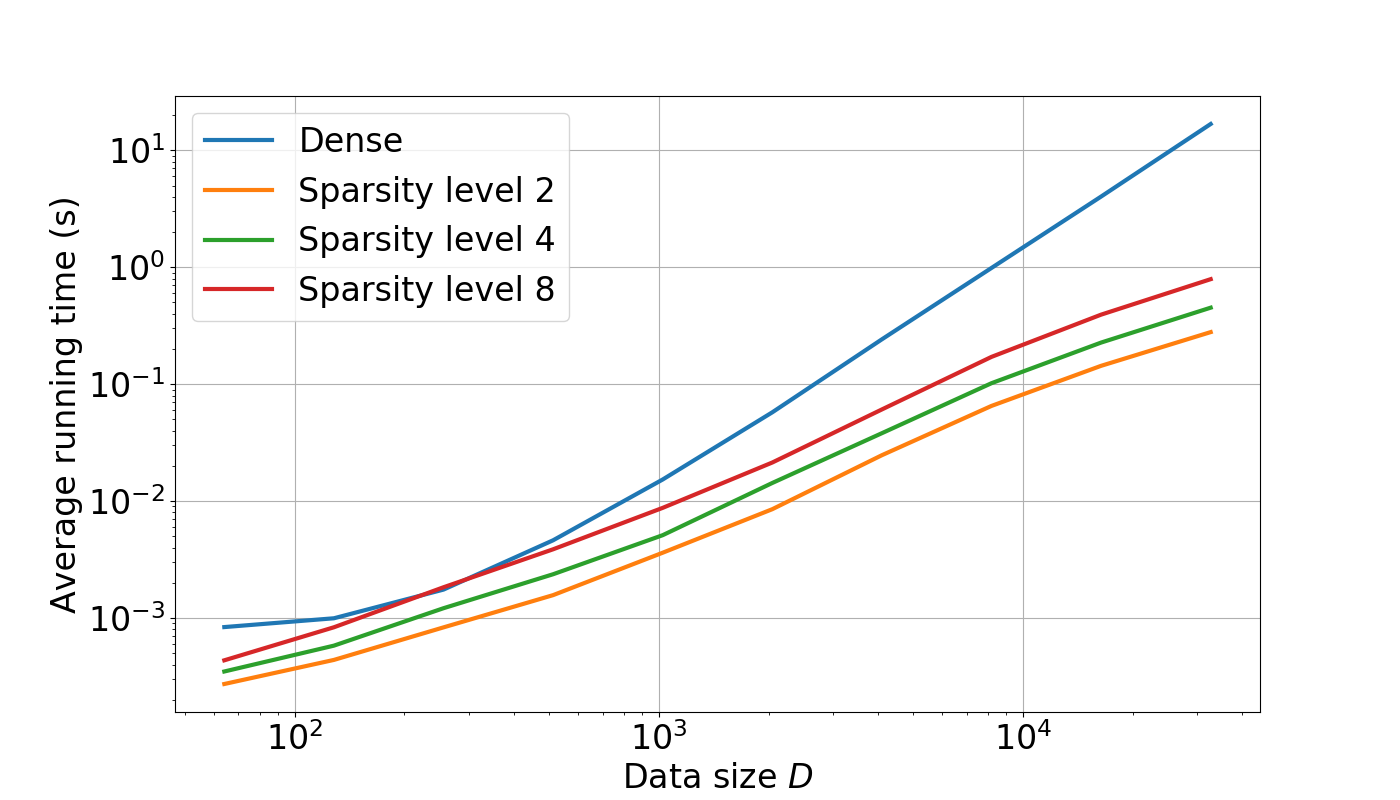
\includegraphics[width=.8\textwidth]{RunningTime4VaryingSparsity.png}
\caption{Running times, averaged over 30 runs, when applying dense or fast $\datadim \times \datadim$ operators to a set of 100 random vectors. The number of factors in fast operators equals $\log_2\left (\datadim\right )$ and the sparsity level denotes the number of non-zero coefficients per row and per column in each factor.}
\label{fig:time_csr}
\end{figure}

%\begin{figure}[tbh]
%\centering
%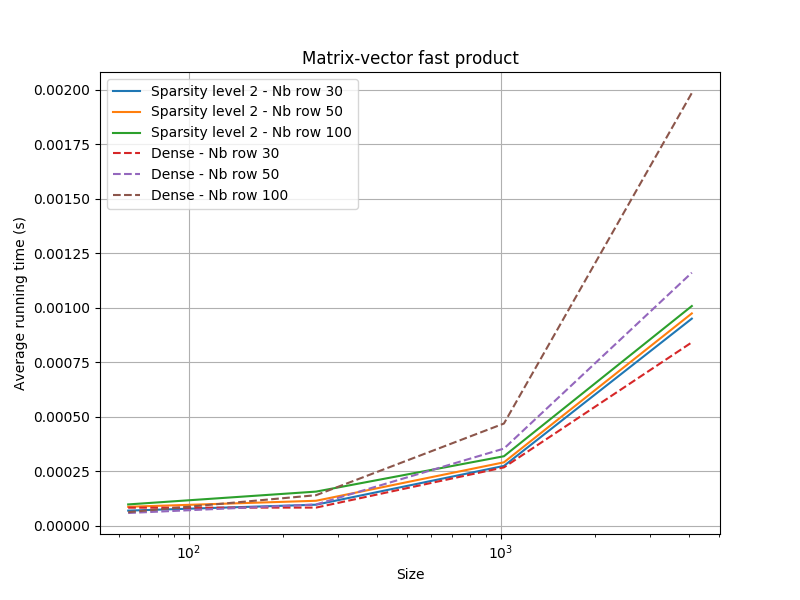
\includegraphics[width=.8\textwidth]{Run_time_sparsity_2.png}
%\caption{Running times, averaged over 30 runs, when applying dense or product of fast operators to a set of 100 random vectors. The number of factors in fast operators equals $\log_2\left (\#~row\right )$ and the sparsity level denotes the number of non-zero coefficients per row and per column in each factor.}
%\label{fig:time_csr_fixed_row_size}
%\end{figure}


\paragraph{Datasets.}
We present results on real-world and toy datasets summarized in Table \ref{table:data}. On the one hand, the real world datasets \texttt{MNIST}~\cite{lecun-mnisthandwrittendigit-2010} and \texttt{Fashion-Mnist}~\cite{Pedregosa2011Scikit} %and \texttt{Labeled Faces in the Wild}~\cite{Huang07e.:labeled} (\texttt{LFW}) 
are used to show --- quantitatively and qualitatively --- the good quality of the obtained centroids when using our method \qkmeans. On the other hand, we use the \texttt{blobs} synthetic dataset from \texttt{sklearn.dataset} to show the speed up offered by our method \qkmeans when the number of clusters and the dimensionality of the data are sufficiently large.
%The code of our method \qkmeans is available on request and will be available online soon. \addLG{je serais d'avis de ne pas dire ça mais soit de dire qu'il est déjà disponible, soit de ne rien dire. Sachant qu'on ne peut pas dire qu'il est déjà disponible en ligne avant le processus de reviewing}


\begin{table*}[!h]
\centering
\begin{tabular}{|c|c|c|c|c|c|}
\hline
\textbf{Dataset} & \textbf{Data dim.} $\datadim$        & \textbf{\# classes} & \textbf{Training set size} $\nexamples$ & \textbf{Test set size} $\nexamples'$ \\ \hline
MNIST                   & 784   & 10        & 60 000    & 10 000               \\ \hline
Fashion-MNIST           & 784   & 10        & 60 000    & 10 000               \\ \hline
% LFW                     & 1850  & 2529      & 8866      & N/A               \\ \hline
Blobs (clusters std: 12)   & 2000  & 1000      & 29000      & 1000               \\ \hline
\end{tabular}
\caption{Datasets statistics}
\label{table:data}
\end{table*}


\paragraph{Algorithm settings.} 
The \qkmeans algorithm is used with $Q\eqdef\log_2\left (A\right )$ sparse factors, where  $A=\min\left (\nclusters, \datadim\right )$. 
All factors $\rmS_q$ are with shape $A \times A$ except, depending on the shape of $\rmA$, the leftmost one ($\nclusters\times A$) or the rightmost one ($A\times\datadim$). 
The sparsity constraint of each factor $\rmS_q$ is set in $\mathcal{E}_q$ and is governed by a global parameter denoted as \textit{sparsity level}, which indicates the desired number of non-zero coefficients in each row and in each column of $\rmS_q$. 
Since the projection onto this set of structured-sparsity constraints may be computationally expensive, this projection is relaxed in the implementation of \palm and only guarantees that the number of non-zero coefficients in each row and each column is at least the sparsity level, as in~\cite{LeMagoarou2016Flexible}.
The actual number of non-zero coefficients in the sparse factors is measured at the end of the optimization process and reported in the results.
The sparse factors are updated using the \palm rather than its hierarchical version, since we observed that this was a better choice in terms of computational cost, with satisfying approximation results (See Figure~\ref{fig:mnist:objfun}~and~\ref{fig:fmnist:objfun}).
Additional details about \palm are given in Appendix~\ref{sec:app:palm4msa}.
The stopping criterion of \kmeans and \qkmeans consists of a tolerance set to $10^{-6}$ on the relative variation of the objective function and a maximum number of iterations set to 10 for the \texttt{Blobs}dataset and to 20 for others. The same principle governs the stopping criterion of \palm with a tolerance set to $10^{-6}$ and a maximum number of iterations set to 300. Each experiment have been replicated using different seed values for random initialisation. Competing techniques share the same seed values, hence share the same initialisation of centroids.

%\subsection{Sparse factors multiplication}
%
%\subsubsection{Sparse factor object}

%\todo[inline]{Parler ici de la configuration de \qkmeans: $Q\eqdef\log_2\left (A\right )$, critère d'arrêt (nombre d'itération, tolérance), ordre des mises à jours, palm4msa plutôt que la version hiérarchique, taille des matrices $\rmS_q$, scaling coefficient, définition de 	$\mathcal{E}_q$.
%}

\subsection{Clustering}

\begin{figure}
\begin{subfigure}[b]{.49\textwidth}
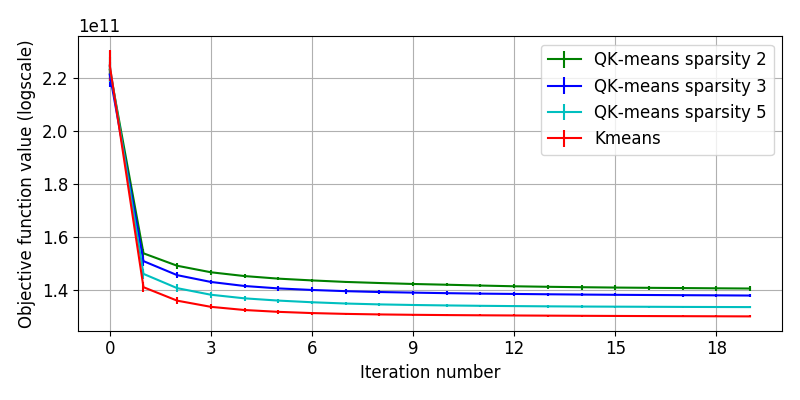
\includegraphics[width=\textwidth]{mnist30_objective.png}
\caption{MNIST, $\nclusters=30$: objective function.}
\label{fig:mnist:objfun}
\end{subfigure}
\begin{subfigure}[b]{.49\textwidth}
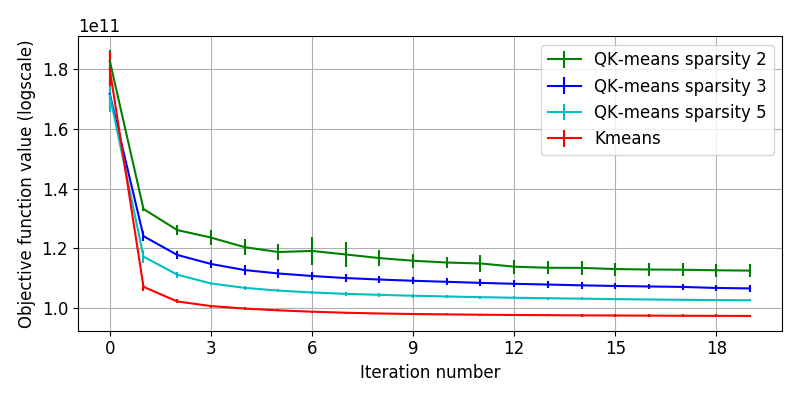
\includegraphics[width=\textwidth]{fashmnist30_objective.png}
\caption{Fashion-MNIST, $\nclusters=30$: objective function.}
\label{fig:fmnist:objfun}
\end{subfigure}
\begin{subfigure}[t]{.49\textwidth}
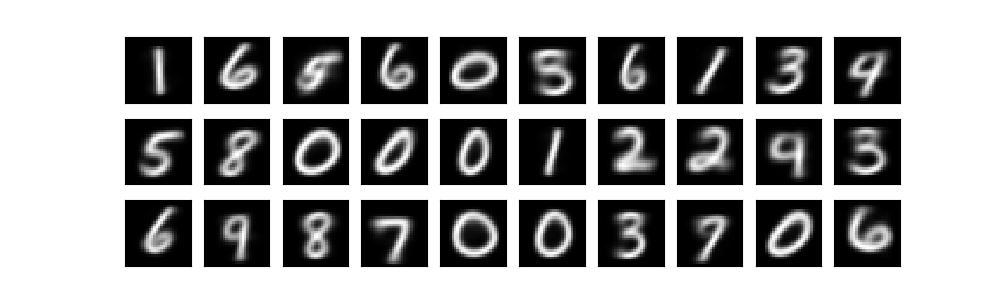
\includegraphics[width=\textwidth]{mnist30_kmeans_centroids.png}
\caption{\kmeans centroids.}
\label{fig:mnist:kmeans:centroids}
\end{subfigure}
\begin{subfigure}[t]{.49\textwidth}
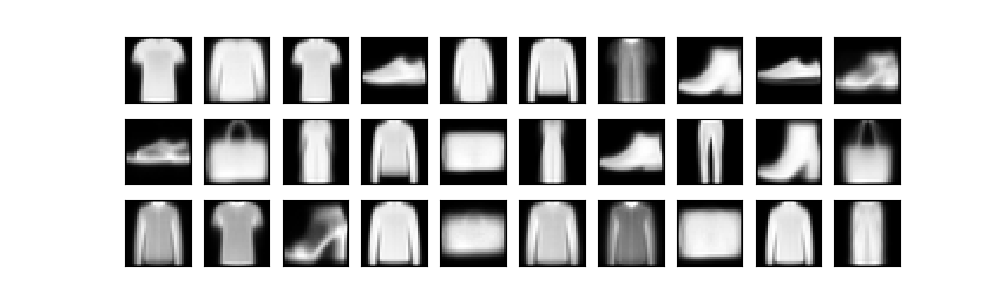
\includegraphics[width=\textwidth]{fashmnist30_kmeans_centroids.png}
\caption{\kmeans centroids.}
\label{fig:fmnist:kmeans:centroids}
\end{subfigure}
\begin{subfigure}[t]{.49\textwidth}
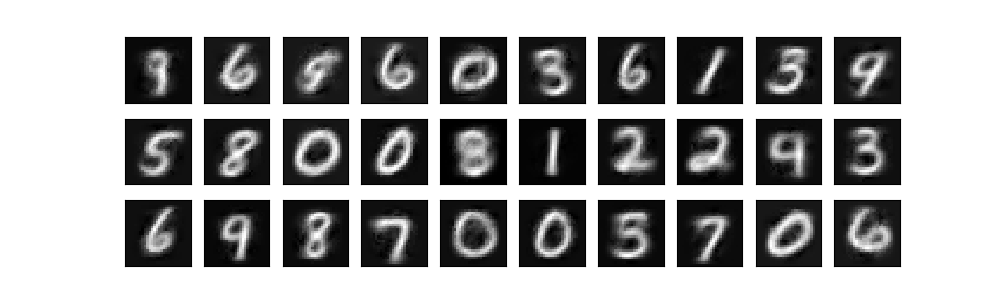
\includegraphics[width=\textwidth]{mnist30_qkmeans_centroids.png}
\caption{\qkmeans centroids.}
\label{fig:mnist:qkmeans:centroids}
\end{subfigure}
\begin{subfigure}[t]{.49\textwidth}
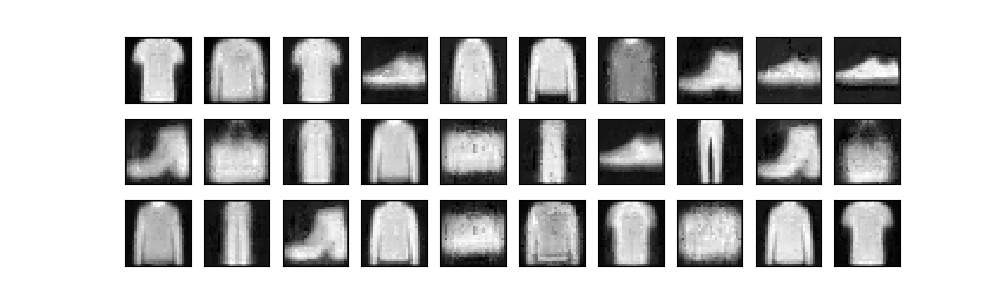
\includegraphics[width=\textwidth]{fashmnist30_qkmeans_centroids.png}
\caption{\qkmeans centroids.}
\label{fig:fmnist:qkmeans:centroids}
\end{subfigure}
\begin{subfigure}[t]{.49\textwidth}
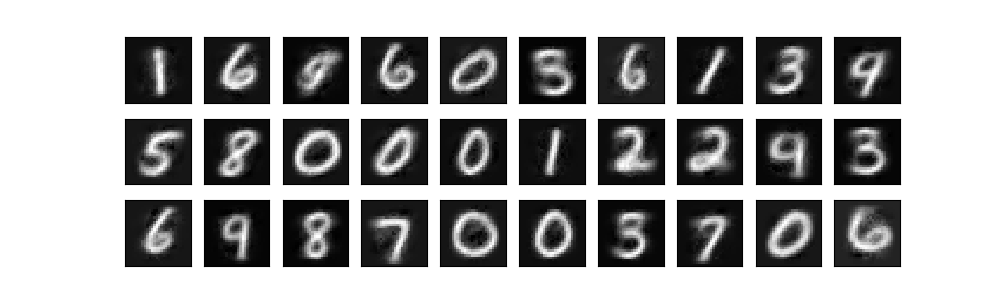
\includegraphics[width=\textwidth]{mnist30_hqkmeans_centroids.png}
\caption{Hierarchical-\palm \qkmeans centroids.}
\label{fig:mnist:hqkmeans:centroids}
\end{subfigure}
\begin{subfigure}[t]{.49\textwidth}
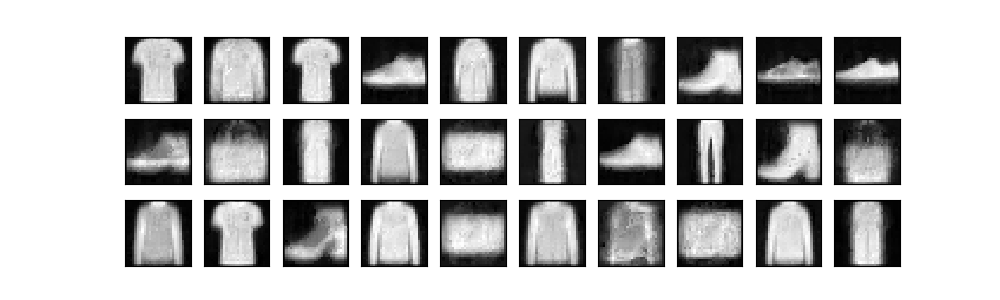
\includegraphics[width=\textwidth]{fashmnist30_hqkmeans_centroids.png}
\caption{Hierarchical-\palm \qkmeans centroids.}
\label{fig:fmnist:hqkmeans:centroids}
\end{subfigure}
\caption{Clustering results on MNIST (left) and Fashion-MNIST (right) for $\nclusters=30$ clusters.}
\label{fig:clustering:realdata}
\end{figure}

\paragraph{Approximation quality.} One important question is the ability of the fast-structure model to fit arbitrary data.
Indeed, no theoretical result about the expressivity of such models is currently available.
In order to assess this approximation quality, the MNIST and Fashion-MNIST data have been clustered into $\nclusters=30$ clusters by \kmeans, \qkmeans and a variant of \qkmeans using the hierarchical version of \palm, with several sparsity levels.
Results are reported in Figure~\ref{fig:clustering:realdata}.
In Figures~\ref{fig:mnist:objfun} and~\ref{fig:fmnist:objfun}, one can observe that the objective function of \qkmeans is decreasing in a similar way as \kmeans over iterations.
In particular, the use of the fast-structure model does not seem \addLG{(to delay the plateau of the objective function)} to slow the procedure down.
At the end of the iterations, the value of objective function for \qkmeans is slightly above that of \kmeans.
As expected, the sparser the model, the more degradation in the objective function.
However, even very sparse models do not degrade the results significantly. These Figures also demonstrate the convergence property of the \qkmeans algorithm when using the standard, proved convergent, \textit{Palm4MSA} algorithm: in this case, the objective function is always non-increasing whereas the \qkmeans version with \textit{Hiearchical Palm4MSA}, not guaranteed to converge, suffers a small bump in its objective function (see Figure~\ref{fig:fmnist:objfun} iteration~6).
The approximation quality can be assessed visually, in a more subjective and interpretable way, in Figures~\ref{fig:mnist:kmeans:centroids} to~\ref{fig:fmnist:hqkmeans:centroids} where the obtained centroids are displayed as images.
Although some degradation may be observed in some images, one can note that each image obtained with \qkmeans clearly represents a single visual item without noticeable interference with other items.

\paragraph{Clustering assignation times.}
Higher dimensions are required to assess the computational benefits of the proposed approach, as shown here.
The assignation times of the clustering procedure were measured on the \texttt{Blobs} dataset.
The centroid matrices are with shape $\nclusters \times \datadim$ with $\datadim=2000$  and $\nclusters\in\left \lbrace 128, 256, 512\right \rbrace$.
Results reported in Figure~\ref{fig:clustering:blobs:assignation_time} show that in this setting and with the current implementation, the computational advantage of \qkmeans is observed in high dimension, for $\nclusters=256$ and $\nclusters=512$ clusters. It is worth noticing that when $K$ increases, the running times are not affected that much for \qkmeans while it significantly grows for \kmeans. These trends are directly related to the number of model parameters that are reported in the figure.


%\todo[inline]{Montrer ensuite les temps d'assignation en mode batch 5000 sur blobs, cf. Figure~\ref{fig:clustering:blobs:assignation_time}. Objectif: montrer qu'à partir d'une certaine dimension, \qkmeans est plus rapide.}
%on-line\footnote{Anonymous URL.}.

\begin{figure}[tbh]
\centering
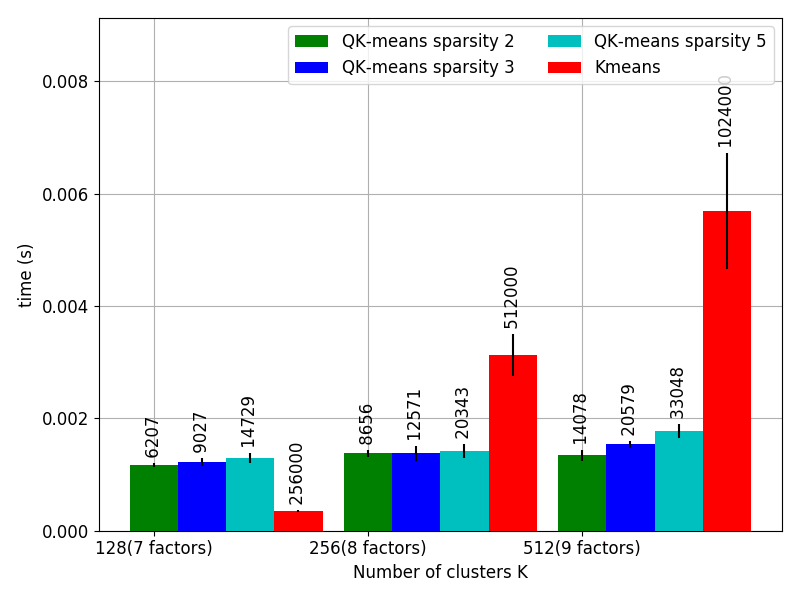
\includegraphics[width=.8\textwidth]{blobs_assignation_time.png}
\caption{Clustering Blobs data: running times of the assignation step, averaged over 5 runs. The vertical black lines are the standard deviation w.r.t. the runs and the average number of parameters actually learned  in the models are reported above those lines.\addVE{to be completed}.}
\label{fig:clustering:blobs:assignation_time}
\end{figure}

\subsection{Nearest-neighbor search in a large dataset}
The Nearest-neighbor search is a fundamental task that suffers from computational limitations when the dataset is large.
Fast strategies have been proposed, e.g., using kd trees or ball trees.
One may also use a clustering strategy to perform an approximate nearest-neighbor search: the query is first compared to $\nclusters$ centroids computed beforehand by clustering the whole dataset, and the nearest neighbor search is then performed among a lower number of data points, within the related cluster.
We compare this strategy using \kmeans and \qkmeans against the \texttt{scikit-learn} implementation~\cite{Pedregosa2011Scikit} of the nearest-neighbor search (brute force search, kd tree, ball tree).
Inference time results on the \texttt{Blobs} dataset are reported in Figure~\ref{fig:nn:blobs} and accuracy results are displayed in Table~\ref{table:results_blobs}. 
% As shown in Figure~\ref{fig:nn:blobs:accuracy}, the accuracy of the approximate nearest neighbor search is above $0.99$ \todo{Accuracy $>0.99$ to be checked} for all the tested variants of \qkmeans, which is an solid evidence about the reliability of the approach.
The running times reported in Figure~\ref{fig:nn:blobs} show a dramatic advantage of using a clustering-based approximate search \todo{to be completed by reporting the actual acceleration ratio obtained by \qkmeans over the three sklearn options.} and this advantage is even stronger with the clustering obtained by our \qkmeans method. This speed-up comes at a cost though, we can see a drop in classification performance in Table~\ref{table:results_blobs}. 

\begin{figure}[tbh]
\centering
%\begin{subfigure}[b]{.49\textwidth}
%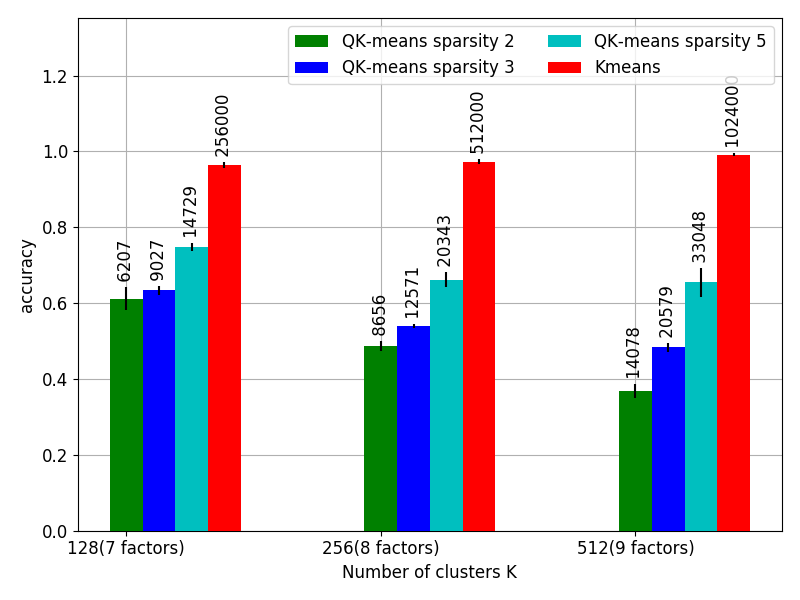
\includegraphics[width=\textwidth]{blobs_1nn_accuracy.png}
%\caption{Accuracy.}
%\label{fig:nn:blobs:accuracy}
%\end{subfigure}
%\begin{subfigure}[b]{.49\textwidth}
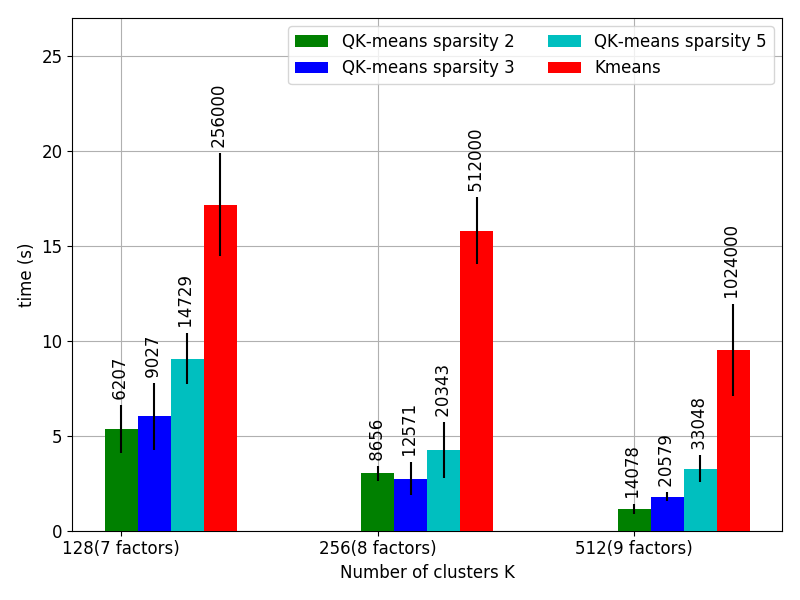
\includegraphics[width=\textwidth]{blobs_1nn_inference_time.png}
%\caption{Running times.}
\label{fig:nn:blobs:times}
%\end{subfigure}

\caption{Running time of nearest neighbor search on blobs data. Results are averaged over 5 runs (vertical lines: standard deviation) and the average number of parameters actually learned is reported above each bar. The results for the Brute Force Search, KD Tree and Ball Tree are not displayed because they were longer than 10 times the K-means search version.}
\label{fig:nn:blobs}
\end{figure}

 
\begin{table}[]

\centering
\begin{tabular}{@{}l|P{2.5cm}}
\toprule
                                    & Accuracy \texttt{Blobs} \\ \midrule
1NN Brute force search              & N/A   \\
1NN KD Tree                         & N/A   \\
1NN Ball Tree                       & N/A   \\ \midrule \midrule
1NN K-means 128 Clusters            & 0.96      \\
1NN K-means 256 Clusters            & 0.97      \\
1NN K-means 512 Clusters            & 0.99      \\ \midrule
1NN QK-means 128 Clusters           & 0.74     \\
1NN QK-means 256 Clusters           & 0.66      \\
1NN QK-means 512 Clusters           & 0.66      \\ \midrule \midrule
Nyström K-means + SVM 128 Clusters  & 0.98      \\
Nyström K-means + SVM 256 Clusters  & 1.0      \\
Nyström K-means + SVM 512 Clusters  & 1.0      \\ \midrule
Nyström QK-means + SVM 128 Clusters & 0.95      \\
Nyström QK-means + SVM 256 Clusters & 1.0      \\
Nyström QK-means + SVM 512 Clusters & 1.0      \\ \bottomrule
\end{tabular}

\caption{Results on the classification task on \texttt{Blobs} dataset. Results are averaged over 5 runs. ``N/A'' denotes experiments that did not finish. Only results with sparsity value 5 are displayed for \qkmeans experiments. For the \qkmeans results, only those obtained with sparsity level = 5 are displayed.}
\label{table:results_blobs}

\end{table}

\begin{table}[]

\centering
\begin{tabular}{@{}l|P{2.5cm}|P{2.5cm}}
\toprule
                                    & Accuracy \texttt{Fashion-MNIST} & Accuracy \texttt{MNIST} \\ \midrule
1NN Brute force search              &  0.85   &  0.97 \\
1NN KD Tree                         & 0.85  &  0.97  \\
1NN Ball Tree                       & 0.85  &  0.97  \\ \midrule \midrule
1NN K-means 10 Clusters            & 0.84  &  0.96  \\
1NN K-means 16 Clusters            & 0.84  &  0.96  \\
1NN K-means 30 Clusters            & 0.84  &  0.96  \\ \midrule
1NN QK-means 10 Clusters           & 0.84  &  0.96  \\
1NN QK-means 16 Clusters           & 0.84  &  0.96  \\
1NN QK-means 30 Clusters           & 0.84  &  0.96  \\ \midrule \midrule
Nyström K-means + SVM 10 Clusters  &  0.71  & 0.74  \\
Nyström K-means + SVM 16 Clusters  &  0.75  & 0.83  \\
Nyström K-means + SVM 30 Clusters  &  0.78  & 0.88  \\ \midrule
Nyström QK-means + SVM 10 Clusters &  0.71  & 0.74  \\
Nyström QK-means + SVM 16 Clusters &  0.74  & 0.82  \\
Nyström QK-means + SVM 30 Clusters &  0.77  & 0.88  \\ \bottomrule
\end{tabular}

\caption{Results on the classification task on the \texttt{MNIST} and \texttt{Fashion-MNIST} datasets. Results are averaged over 5 runs. ``N/A'' denotes experiments that did not finish. For the \qkmeans results, only those obtained with sparsity level = 5 are displayed.}
\label{table:results_mnist_fmnist}

\end{table}

\subsection{Nyström approximation}

In this sub-section, we show how we can take advantage of the fast-operator obtained as output of our \qkmeans algorithm in order to speed-up the computation in the Nyström approximation. 
We start by giving background knowledge on the Nyström approximation then we present some recent work aiming at accelerating it using well know fast-transform method. 
We finally stem on this work to present a novel approach based on our \qkmeans algorithm.

\subsubsection{Background on the Nyström approximation}

Standard kernel machines are often impossible to use in large-scale applications because of their high computational cost associated with the kernel matrix $\rmK$ which has $O(n^2)$ storage and $O(n^2d)$ computational complexity: $\forall i,j \in\intint{\nexamples}, \rmK_{i,j} = k(\rvx_i, \rvx_j)$. A well-known strategy to overcome this problem is to use the Nyström method which computes a low-rank approximation of the kernel matrix on the basis of some pre-selected landmark points. 

Given $K \ll n$ landmark points $\{\rmU_i\}_{i=1}^{K}$, the Nyström method gives the following approximation of the full kernel matrix:
%
\begin{equation}
 \label{eq:nystrom}
 \rmK \approx \tilde\rmK = \rmC\rmW^\dagger\rmC^T,
\end{equation}
%
with $\rmW \in \R^{K \times K}$ containing all the kernel values between landmarks: $\forall i,j \in [\![K]\!]~ \rmW_{i,j} = k(\rmU_i, \rmU_j)$; $\rmW^\dagger$ being the pseudo-inverse of $\rmW$ and $\rmC \in \R^{n \times K}$ containing the kernel values between landmark points and all data points: $\forall i \in [\![n]\!], \forall j \in [\![K]\!]~ \rmC_{i, j} = k(\rmX_i, \rmU_j)$.

\subsubsection{Efficient Nyström approximation}

A substantial amount of research has been conducted toward landmark point selection methods for improved approximation accuracy \cite{kumar2012sampling} \cite{musco2017recursive}, but much less has been done to improve computation speed. In \cite{si2016computationally}, the authors propose an algorithm to learn the matrix of landmark points with some structure constraint, so that its utilisation is fast, taking advantage of fast-transforms. This results in an efficient Nyström approximation that is faster to use both in the training and testing phases of some ulterior machine learning application.

Remarking that the main computation cost of the Nyström approximation comes from the computation of the kernel function between the train/test samples and the landmark points, \cite{si2016computationally} aim at accelerating this step. In particular, they focus on a family of kernel functions that has the following form:
%
\begin{equation}
 k(\rvx_i, \rvx_j) = f(\rvx_i) f(\rvx_j) g(\rvx_i^T\rvx_j),
\end{equation}
%
where $f: \R^d \rightarrow \R$ and $g: \R \rightarrow \R$. They show that this family of functions contains some widely used kernels such as the Gaussian and the polynomial kernel. Given a set of $K$ landmark points $\rmU \in \R^{K \times d}$ and a sample $\rvx$, the computational time for computing the kernel between $\rvx$ and each row of $\rmU$ (necessary for the Nyström approximation) is bottlenecked by the computation of the product $\rmU\rvx$. They hence propose to write the $\rmU$ matrix as the concatenation of structured $s = K / d$ product of matrices:
%
\begin{equation}
 \rmU = \left[ \rmV_1 \rmH^T, \cdots, \rmV_s\rmH^T  \right]^T,
\end{equation}
%
where the $\rmH$ is a $d \times d$ matrix associated with a fast transform such as the \textit{Haar} or \textit{Hadamard} matrix, and the $\rmV_i$s are some $d \times d$ diagonal matrices to be either chosen with a standard landmark selection method or learned using an algorithm they provide.

Depending on the $\rmH$ matrix chosen, it is possible to improve the time complexity for the computation of $\rmU\rvx$ from $O(Kd)$ to $O(K \log{d})$ (\textit{Fast Hadamard transform}) or $O(K)$ (\textit{Fast Haar Transform}).

\subsubsection{\qkmeans in Nyström}

We propose to use our \qkmeans algorithm in order to learn directly the $\rmU$ matrix in the Nyström approximation so that the matrix-vector multiplication $\rmU \rvx$ is cheap to compute, but the structure of $\rmU$ is not constrained by some pre-defined transform matrix. We propose to take the objective $\rmU$ matrix as the \kmeans matrix of $\rmX$ since it has been shown to achieve good reconstruction accuracy in the Nyström method \cite{kumar2012sampling}.

As shown in the next sub-section, our algorithm allow to obtain an efficient Nyström approximation, while not reducing too much the quality of the \kmeans landmark points which are encoded as a factorization of sparse matrix. 

\subsubsection{Results}

The Figure~\ref{fig:nystrom} summarizes the results achieved in the Nyström approximation setting. 

The Figures on the right display the average time for computing one line of the approximated matrix in Equation~\ref{eq:nystrom}. In Figure~\ref{fig:blobs:nystrom_time}, we clearly see the speed-up offered using the \qkmeans method on the \texttt{Blobs} dataset. On the \texttt{Mnist} and \texttt{Fashion-MNIST} dataset (Figure~\ref{fig:mnist:nystrom_time}~and~\ref{fig:fashmnist:nystrom_time}), this speed-up is sensible but not as clear because the standard deviation is much larger. 

The Figures on the left show the approximation error of the Nyström approximation based on different sampling schemes w.r.t. the real kernel matrix. This error is computed by the Froebenius norm of the difference between the matrices and then normalized:

\begin{equation}
 error = \frac{||\rmK - \tilde\rmK||_F}{||\rmK||_F}
\end{equation}

. The \qkmeans approach gives better reconstruction error than the Nyström method based on uniform sampling although they are slightly worse than the one obtained with the \kmeans centroids. We see that that the difference in approximation error between \kmeans and \qkmeans is almost negligeable when compared to the approximation error obtained with the uniform sampling scheme.

From a more practical point of view, we show in Table~\ref{table:results_blobs} and Table~\ref{table:results_mnist_fmnist} that the Nyström approximation based on \qkmeans can then be used in a linear SVM and achieve as good performance as the one based on the \kmeans approach.


\begin{figure}
\begin{subfigure}[b]{.49\textwidth}
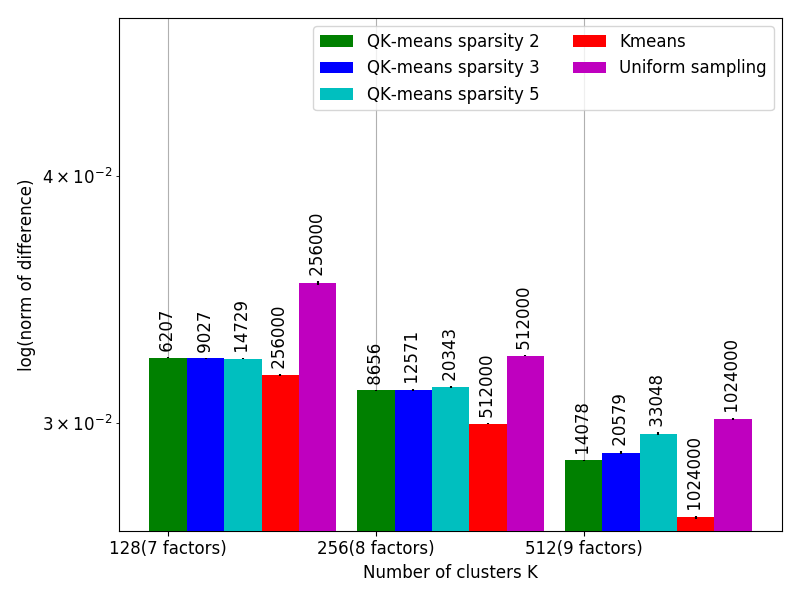
\includegraphics[width=\textwidth]{blobs_nystrom_error.png}
\caption{\texttt{Blobs}: Nyström reconstruction error.}
\label{fig:blobs:nystrom_error}
\end{subfigure}
\begin{subfigure}[b]{.49\textwidth}
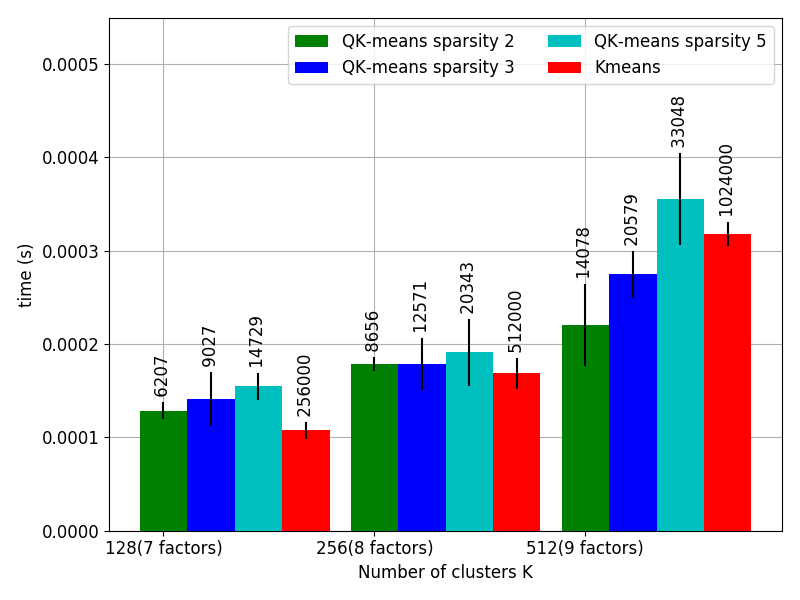
\includegraphics[width=\textwidth]{blobs_nystrom_inference_time.png}
\caption{\texttt{Blobs}: Nyström inference time.}
\label{fig:blobs:nystrom_time}
\end{subfigure}
\begin{subfigure}[b]{.49\textwidth}
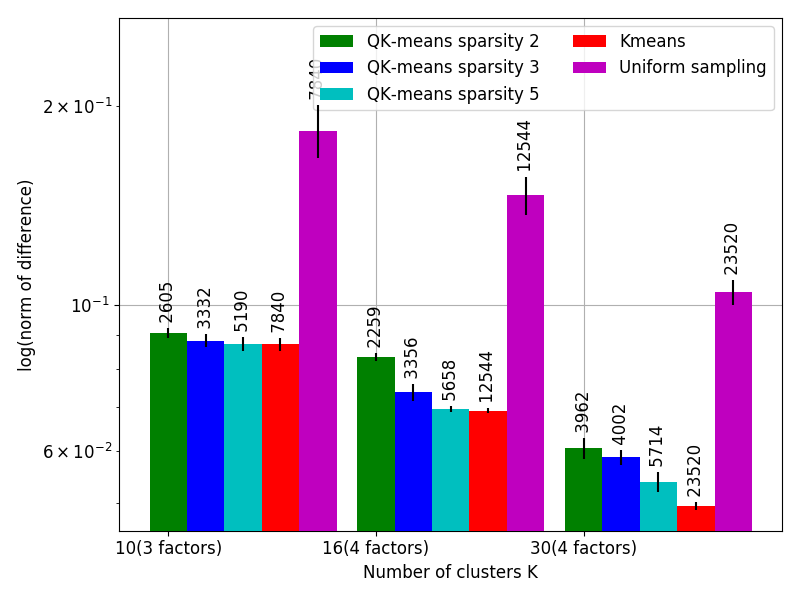
\includegraphics[width=\textwidth]{mnist_nystrom_error.png}
\caption{\texttt{MNIST}: Nyström reconstruction error.}
\label{fig:mnist:nystrom_error}
\end{subfigure}
\begin{subfigure}[b]{.49\textwidth}
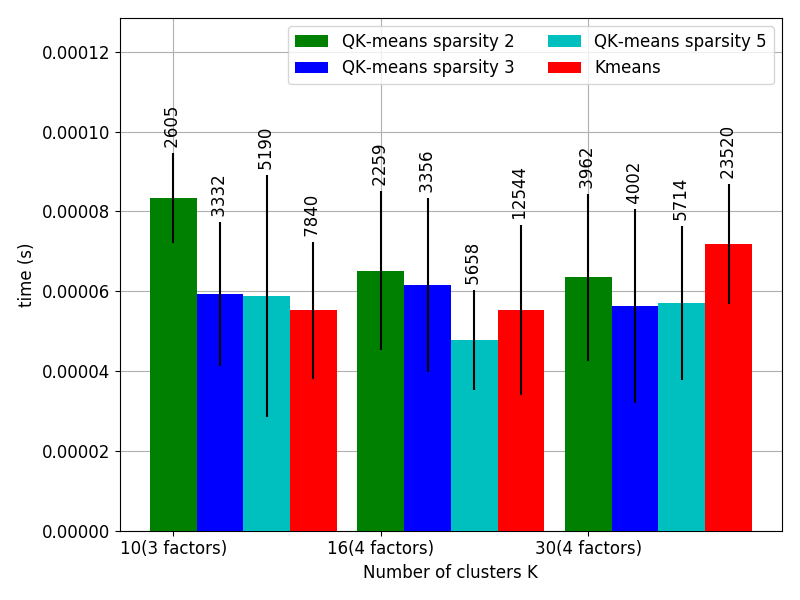
\includegraphics[width=\textwidth]{mnist_nystrom_inference_time.png}
\caption{\texttt{MNIST}: Nyström inference time.}
\label{fig:mnist:nystrom_time}
\end{subfigure}
\begin{subfigure}[b]{.49\textwidth}
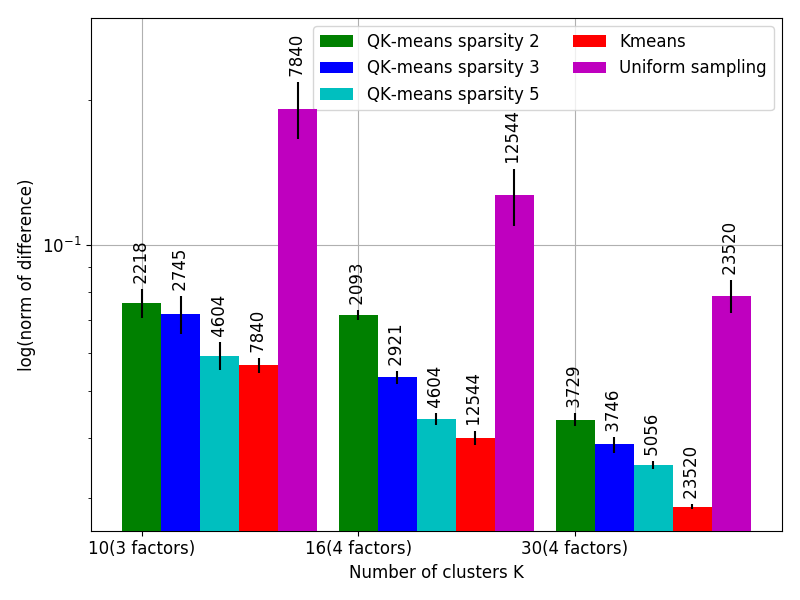
\includegraphics[width=\textwidth]{fashmnist_nystrom_error.png}
\caption{\texttt{Fashion-MNIST}: Nyström reconstruction error.}
\label{fig:fashmnist:nystrom_error}
\end{subfigure}
\begin{subfigure}[b]{.49\textwidth}
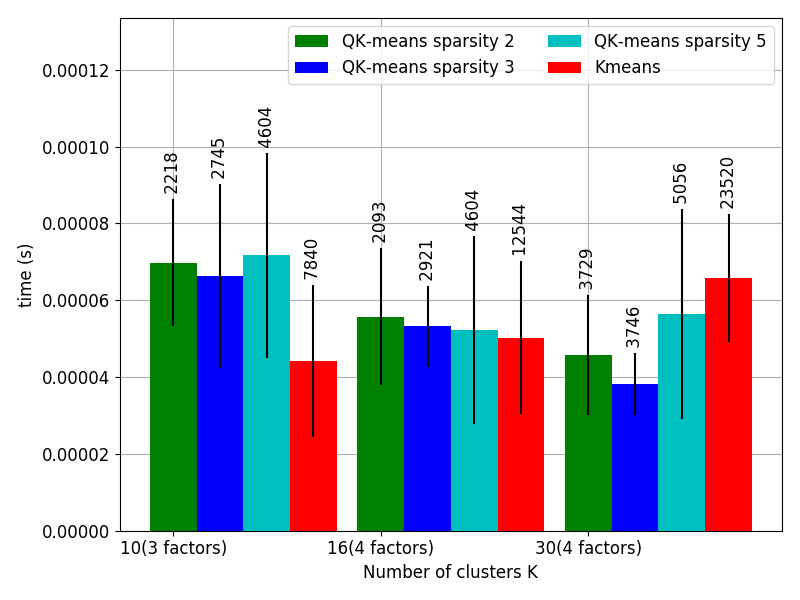
\includegraphics[width=\textwidth]{fashmnist_nystrom_inference_time.png}
\caption{\texttt{Fashion-MNIST}: Nyström inference time.}
\label{fig:fashmnist:nystrom_time}
\end{subfigure}
\caption{Nystr\"om approximation results: accuracy (left) and running times (right). The uniform sampling based Nyström approximation running times are not displayed because they are the same as for the Nyström approximation based on \kmeans centroids. Every experiment results are averaged over 5 runs. The vertical black lines are the standard deviation w.r.t. the runs.}
\label{fig:nystrom}
\end{figure}

%{RBF networks}

%Besoin d'éclaircir les liens avec RBF networks

%\subsection{nearest-neighbours}

%Besoin d'éclaircir les liens avec nearest neighbours

\section{Conclusion}
\label{sec:conclusion}

In this paper, we proposed a new algorithm with convergence proof, that allows to learn a matrix of K-means center-points with sparse factorization constraint. We provide complexity analysis showing, that this particular matrix may speed up further machine learning algorithms that would usually make use of the standard K-means center-point matrix. In particular, we show that this algorithm could be used in the context of the Nyström approximation.

This paper does not contain any experimental results as it describes ongoing work. In the following, %next subsection (Section \ref{sec:foreseen_experiments}), 
we discuss foreseen experiments that would aim at illustrating the speed gain when using our method, while not reducing the overall accuracy in machine learning settings.
%
%Last but not least, we discuss in the Section \ref{sec:discussion} 
We also discuss a broader scope of application of our algorithm and some possible theoretical advantages.

\subsection{Foreseen experiments}
\label{sec:foreseen_experiments}

Our algorithm will be evaluated on the same metrics than \cite{si2016computationally} on the Nyström approximation, namely the reconstruction error of the kernel matrix and the accuracy error in subsequent machine learning experiments. Those errors will be considered with respect to the computation speed. The considered baseline will be Nyström with simple K-means selected landmark points and, obviously, the efficient Nyström algorithm proposed in \cite{si2016computationally}.

\subsection{Discussion}
\label{sec:discussion}

The algorithm we propose, \textit{Q-means}, could be applied to any other method that uses the K-means algorithm in its initialization. The K-means Nyström method is only one instance of such algorithm but we can already think of other examples, such as some nearest neighbour search algorithm based on the K-means clustering of the input space \cite{wang2011fast}.

Finally, the sparse factorization constraint for the K-means center point matrix may play the role of a regularization, with parameter being the number of values in each factor. 
We wish to investigate also this property more thoroughly from both theoretical and experimental point of view.
%This is just an intuition for now and this must be investigated more thoroughly from both the theoretical and experimental point of view.

%\begin{itemize}
% \item rbf networks
% \item hierarchical nearest neighbours
%\end{itemize}

%====================================================================================

\bibliography{biblio}
\bibliographystyle{aaai}


\end{document}
